\documentclass{article}
\usepackage[utf8]{inputenc}
\usepackage{CJKutf8}
\usepackage{enumitem}
\usepackage{hyperref}
\usepackage{geometry}
\usepackage{longtable}
\usepackage{booktabs}
\usepackage{xcolor}
\usepackage{amsmath}
\usepackage{graphicx}
\usepackage{amssymb}
\usepackage{float}
\renewcommand{\v}[1]{ \ensuremath{ {\mathbf{#1}} }} 
\geometry{a4paper, margin=1in}
\DeclareMathOperator{\Cov}{Cov}   % Add this
\DeclareMathOperator{\Var}{Var}   % Optional, for consistency
\DeclareMathOperator{\E}{E}       % Optional, for expectation
% Custom verbatim for file trees (avoids lstlisting issues)
\newcommand{\filetree}[1]{
  \vspace{1em}
  \begingroup
  \ttfamily\small
  \begin{tabular}{@{}l@{}}
    #1
  \end{tabular}
  \endgroup
  \vspace{1em}
}



\begin{document}

\title{Particle Flow Filter and Differentiable Particle Filter}

\author{Haowu Duan}



%\begin{abstract}\end{abstract}


\maketitle

\tableofcontents

%%%%%%%%%%%%%%%%%%%%%%%%%%%%%%%%%%%%%%%%%%%%%%%%%%%%%%%%%%
\newpage
\section{Literature Review}

\subsection{State-Space Modeling in Financial Markets: The Big Picture}
Financial systems are driven by latent factors that shape observable market data. Problems such as stochastic volatility, limit order book dynamics, or macroeconomic regime shifts are frequently cast as Hidden Markov Models (HMMs) or continuous state-space models (SSMs). In quantitative finance, Bayesian filtering and smoothing are key tools for recovering these hidden drivers. A central example is \textit{stochastic volatility} modeling, where asset volatility is a drifting latent state. Recent semi-parametric methods employ particle filters to estimate it without rigid parametric forms, yielding more accurate option pricing and risk management~\cite{feng2025semiparametric}. Discrete state-space models, particularly HMMs, excel at \textit{regime detection}. They treat market regimes (``bull'' vs.\ ``bear'', high vs.\ low momentum) as latent states, enabling traders to estimate real-time regime-shift probabilities and adapt allocations~\cite{catello2023hidden}. Filtering techniques also tackle microstructure noise in \textit{illiquid markets}. Particle filters, for instance, reconstruct the latent ``true'' mid-price of sparsely traded assets (e.g., corporate bonds) from irregular, noisy transaction records~\cite{gueant2018mid}. As a one-dimensional demonstration, let us first write down the state-space model,
\begin{equation}
\begin{split} \label{Eq:HMM}
     x_k &= f(x_{k-1}, w_k) \\
     z_k &= h(x_k, u_k)
\end{split}
\end{equation}
where $k$ denotes the time step, $z_k$ is the observation, and $x_k$ is the unobserved latent state. The noise terms $w_k$ and $u_k$ are mutually and temporally uncorrelated. The function $f$ governs state evolution and $h$ maps the state to observations. In practice we observe only $z_k$, which may have the same or lower dimension than $x_k$ (the latter case is called partial observation and makes inference substantially harder due to information loss). Successful application of state-space models rests on two pillars:
\begin{enumerate}
    \item  A well-specified model with accurate parameters — traditionally this means understanding the functional forms of $f$ and $h$ and estimating their parameters reliably
    \item An effective inference algorithm that estimates the hidden state $x_k$ from the observation $z_k$ — here, a filtering algorithm.
    \end{enumerate}
In recent years, neural networks have entered both parts of the equation. We can replace the conventional maps with learned versions: $f \to f_\theta$ and $h \to h_\theta$. Neural filtering algorithms have also emerged. We will first review the conventional numerical methods, then discuss possible ways for improvement leveraging neural networks.

% Financial systems are characterized by latent factors driving observable market data. Whether modeling stochastic volatility, limit order book dynamics, or macroeconomic regime shifts, the underlying problem is often formulated as a Hidden Markov Model (HMM) or a continuous State-Space Model (SSM). 


% In the domain of quantitative finance, Bayesian filtering and smoothing are essential for isolating latent variables that drive market dynamics but cannot be directly observed. A primary application is found in \textit{Stochastic Volatility} modeling, where the underlying volatility of an asset is treated as a hidden state that drifts over time; recent semi-parametric approaches utilize particle filters to estimate these volatility states without forcing rigid parametric assumptions, thereby improving option pricing and risk management accuracy\cite{feng2025semiparametric}
% . 
% Complementary to continuous estimation, discrete state-space models, specifically Hidden Markov Models (HMMs), are widely employed for \textit{Regime Detection}. By treating market conditions (such as ``bull'' vs. ``bear'' phases or high vs. low momentum) as latent states, these models allow algorithmic traders to infer the probability of a regime shift in real-time and adjust portfolio allocations accordingly\cite{catello2023hidden} 
% . 
% Furthermore, these filtering techniques address microstructure noise in \textit{Illiquid Markets}; for instance, particle filters are used to reconstruct the continuous ``true'' mid-price of sparsely traded assets, such as corporate bonds, by processing irregular and noisy transaction data\cite{gueant2018mid}.\\
% As a one dimensional demonstration, let us first write down the State space model,
% \begin{equation}
% \begin{split} \label{Eq:HMM}
%      x_k &= f(x_{k-1}, w_k) \\
%      z_k &= h(x_k, u_k)
% \end{split}
% \end{equation}
% where k will be reserved for time step, $z_k$ is the observation at k and $x_k$ is the latent state that we do not have direct access to. $w_k, u_k$ are two mutually-uncorrelated and temporally-uncorrelated noise. $f$ is the evolution model and $h$ is the observation model. In real life application, we only have access to the observation, which might have the same dimension or lower dimension than the actual ground truth, in which case we call it partial observation. Of course, in such scenario, our job is more difficult due to the significant lost of information.

% There are essentially two component for successful application of State Space Model. The first is a good model with accurate parameters, and the second is a reliable algorithm to deploy the model. Conventionally, a good model means solid understanding of the functional form of $f$ and $h$, including their parameters. The deployment of the model refers to the numerical algorithm that can recover the state $x_k$ based on the observation $z_k$, in this project, it is the filtering algorithms. In recent years, more people have started to use neural networks and machine learning techniques to this problem. Not going into to much details, we can replace the model which is the map from its input to the output with neural networks, $f \rightarrow f_{\theta}$ and $h \rightarrow h_\theta$. There are also neural network based filtering methods. Our goal would be performing the task above efficiently and accurately.


% \subsubsection{The gist of performing filtering}
% Having a good model is only half the battle, we need solid implementation. In the research world, people will develop novel filtering algorithms that can successfully do the "filtering". These research are based on artificially generated data where we know the ground truth therefore have definitive way to test the performance of the model. Given model $f$ and $h$, what we want is to be able to make good estimation about the hidden state $x_k$, which can be accessed through conditional probability $p(x_k|z_{1:k})$. This can be built up based on historical data,
% \begin{equation}
% \begin{split}
%    {\textbf{Prediction:} }&  \;\;\;\; p(x_k | z_{1:k-1}) = \int p(x_k | x_{k-1}) p(x_{k-1} | z_{1:k-1}) \, dx_{k-1}  \\
%    {\textbf{Update:} }& \;\;\;\;  p(x_k | z_{1:k}) = \frac{p(z_k | x_k) p(x_k | z_{1:k-1})}{p(z_k | z_{1:k-1})} 
% \end{split}
% \end{equation}
% By estimation, we don't really mean recover the exact value, because real world dynamics of the financial market for example is not deterministic. The useful quantity is the probability to make the prediction, roughly speaking, the mean $m_k$ and the variance $P_k$. This problem is a path integral which is not tractable even for one dimensional model except rare cases. We will not expand the details too much here, since different filtering method does not share the same mathematical framework or manifestation. The bottom line is that a successful filtering algorithm can make numerically stable estimation about $p(x_k|z_{1:k-1})$ for known models. 
% \subsubsection{Parameter estimation}
% Assuming the algorithm works, we can then use it to fit the parameter of the model. We still need to assume the same functional form but keep the model parameter as variables. A good set of parameter $\{\theta\}$ will describe data well. Which means $p_\theta(z_k:z_{1:k-1})$ is large. The loss function for this optimization problem is the negative log-likelihood.
% \begin{equation}
%     L(\theta)=-\sum_{k=1}^{T} \log p_\theta(z_k:z_{1:k-1})
% \end{equation}
% since log is monotonic increasing function, minimize this loss function indicates high probability (density) for each observation.\cite{Särkkä2013BayesianFilteringAndSmoothing}. If we are doing Bayesian fit, where the parameters were draw from some distribution $p(\theta)$, the loss function is modified as,
% \begin{equation}
%     L(\theta)=-\sum_{k=1}^{T} \log p_\theta(z_k:z_{1:k-1})- \log p(\theta)
% \end{equation}
% this is known as MAP (Maximum A Posteriori) estimation.


\subsubsection{The gist of performing filtering}

Having a good model is only half the battle; we also need a reliable implementation. In research, novel filtering algorithms are developed and evaluated on synthetic data where the ground truth is known, allowing clear performance measurement. Given the state evolution $f$ and observation model $h$, the goal is to estimate the hidden state $x_k$ via the filtering distribution $p(x_k \mid z_{1:k})$. This is obtained recursively:

\begin{equation}
\begin{split}
   \textbf{Prediction: } & \quad p(x_k \mid z_{1:k-1}) = \int p(x_k \mid x_{k-1}) \, p(x_{k-1} \mid z_{1:k-1}) \, dx_{k-1} \\[1ex]
   \textbf{Update: }     & \quad p(x_k \mid z_{1:k}) = \frac{p(z_k \mid x_k) \, p(x_k \mid z_{1:k-1})}{p(z_k \mid z_{1:k-1})}
\end{split}
\end{equation}

In financial applications (and most real-world settings), we do not aim to recover an exact deterministic value of $x_k$. Instead, the useful quantities are typically the mean $m_k$ and covariance $P_k$ of the filtering distribution. The filtering problem is generally a high-dimensional path integral and is intractable except in special cases (e.g., linear Gaussian SSMs). Different filtering methods (EKF, UKF, particle filters, etc.) use distinct approximations and mathematical frameworks. The key requirement for any successful filtering algorithm is that it produces numerically stable and accurate approximations to $p(x_k \mid z_{1:k})$ for known model dynamics.

\subsubsection{Parameter estimation}

Once a reliable filtering algorithm is available, it can be used to estimate the model parameters $\theta$. We retain the functional forms of $f$ and $h$ but treat their parameters as variables to be learned. A good parameter set $\{\theta\}$ should assign high probability to the observed sequence. This is achieved by maximizing the marginal likelihood $p_\theta(z_{1:T})$, or equivalently minimizing the negative log-likelihood:
\begin{equation}
    L(\theta) = -\sum_{k=1}^{T} \log \, p_\theta(z_k \mid z_{1:k-1})
\end{equation}
Since the logarithm is monotonically increasing, minimizing $L(\theta)$ maximizes the predictive density of each observation given past data~\cite{Särkkä2013BayesianFilteringAndSmoothing}. In a Bayesian setting, where parameters are given a prior $p(\theta)$, we instead minimize,
\begin{equation}
    L(\theta) = -\sum_{k=1}^{T} \log \, p_\theta(z_k \mid z_{1:k-1}) - \log p(\theta),
\end{equation}
which corresponds to maximum a posteriori (MAP) estimation.









% If the evolution and observation is linear, with additive noises, the integral is exactly computable. And we can directly have access to the probability distribution. If the evolution or observation is slightly non-linear, we can try to approximate it with linear model and this is what UKF and EKF does. If there are strong non-linearity, then we need a different approach to compute the integral such as Monte Carlo. 



% To make a simplified demonstration, we can approximate $p(x_{k-1} | z_{1:k-1})$ with a ensemble of particles. 










% The possible source of complication is the following:
% \begin{enumerate}
%     \item $f$ or $h$ is nonlinear.
%     \item Noise distribution is non-Gaussian.
%     \item The curse of dimensionality
% \end{enumerate}
% Each of these three problems poses fundamental challenges for the application of State-Space Model. For us to be able to apply SSM to a real world problem, classically, one makes an ansatz for the model, the filtering step is just to test how well the current parameter choices perform on the data then based on the the target data, we make corrections to the model parameters. {\color{red} Here we can highlight different approach to do it.} But assuming we have a good model, what we want is to be able to make good estimation about the hidden state, namely we want to either compute $p(x_k|z_{1:k})$ directly or have access to its samples. Regardless the approach, there are two steps. 
% \begin{equation}
% \begin{split}
%    {\textbf{Prediction:} }&  \;\;\;\; p(x_k | z_{1:k-1}) = \int p(x_k | x_{k-1}) p(x_{k-1} | z_{1:k-1}) \, dx_{k-1}  \\
%    {\textbf{Update:} }& \;\;\;\;  p(x_k | z_{1:k}) = \frac{p(z_k | x_k) p(x_k | z_{1:k-1})}{p(z_k | z_{1:k-1})} 
% \end{split}
% \end{equation}








% Discuss the nature of financial data:
% - High frequency vs. low frequency
% - Non-stationary, non-Gaussian (fat tails), and non-linear dynamics.
% - The need for sequential inference (online learning) for risk management and algorithmic trading.


\subsection{The Kalman Family and Semi-Exact Methods}
For Linear-Gaussian systems, the Kalman Filter (KF) provides the optimal solution because the product of two Gaussian distributions stays Gaussian. However, financial data rarely satisfies these constraints. Extensions such as the Extended Kalman Filter (EKF) and Unscented Kalman Filter (UKF) utilize linearization and sigma-point approximations, respectively. Either way, for Gaussian distributions, we only need the mean and variance at time $k$, $m_k$ and $P_k$. 
\begin{equation}
\begin{split}
x_k =& f x_{k-1} + w_k, \quad w_k \sim \mathcal{N}(0, Q) \\
z_k =& h x_k + v_k, \quad v_k \sim \mathcal{N}(0, R)
\end{split}
\end{equation}
where $f$ and $h$ are constant in one dimension and matrices in higher dimension. When the kernel becomes non-linear, one essentially expands it around the last input. 
\begin{equation}
\begin{split}
    f(x_{k-1}) &\approx \frac{\partial f(x)}{\partial x} \Big|_{x_{k-1}} \cdot x_{k-1} =f_{k} x_{k-1} \\
    h(x_{k-1}) &\approx \frac{\partial h(x)}{\partial x} \Big|_{x_{k}} \cdot x_{k} =h_{k} x_{k} \\
\end{split}
\end{equation}
This essentially introduces time dependence into the kernels but does not change the Gaussian assumption. This works fine if the higher-order terms are unimportant. UKF uses sigma points to track the mean and variance and is able to capture some higher-order correlations, but it still assumes a Gaussian distribution. Appendix~\ref{APP:Kalman} includes all the details such as key derivations. The Kalman family mostly serves as a benchmark and has very limited application. Both EKF and UKF are methods to overcome the non-linearity in the problem, with more recent progress in this direction \cite{jiang2025new}. However, there are other difficulties as well, notably the curse of dimensionality. Attempts have been made to improve in this direction, notably the Cubature Kalman Filter (CKF)\cite{arasaratnam2009cubature} and Ensemble Kalman Filter (EnKF)\cite{evensen-2003-ensemble-kalman-filter,alghattas2024ensemble}. Here I do want to mention the latest progress on application of neural networks to the Kalman filter, known as KalmanNet\cite{DBLP:journals/corr/abs-2107-10043,mortada2025recursive}. This is a method that replaces the Kalman Gain computation with a learned neural network while keeping everything else from the standard KF flow intact. The key is to train the RNN to make predictions about the Kalman gain without knowing what the noise distribution is. It gets the noise from the input data. While KalmanNet borrows design from the Kalman filter, it can be applied to non-linear, non-Gaussian state space models. 

\subsection{Particle-Based Methods}
Particle-based methods, also known as sequential Monte Carlo, are the focus of this project. They are less model-specific, and therefore more general. There are many different particle-based methods, but the bottom line is how to represent a complicated distribution efficiently. If we were to use particles, namely samples, to represent a distribution $p(x)$, we first need to discretize the phase space.
\begin{equation}
    p(x)=\int dy\; p(y) \delta(y-x)
\end{equation} 
The discretized version is,
\begin{equation}
    p(x)\propto \sum_i \Delta p(x_i) \delta_{x,x_i}= \sum_i \omega_i \delta_{x,x_i}
\end{equation}
where we have evenly sampled the phase space points and give them weights that realize the actual distribution. 
% where $n_i$ is the multiplicity of particle $x_i$. If we treat all the particle in the same footing, then multiplicity will be where we store the distribution, if we give the particle a weight $\omega^i$, then the multiplicity $\tilde n^i$ will be corrected such that $\tilde n^i \omega^i=n^i$. If we pick $\omega^i=n^i$, then particle multiplicity will be trivial. Particle filter methods corresponds to $\omega^i=n^i$ case, namely we don't have identical particles. 
To put this in the context of sequential Monte Carlo, we demonstrate the so-called Bootstrap particle filter (BPF). At step $k$, we have the realization of the distribution $\{x^{(k-1)}_i,\omega^{(k-1)}_i\} \sim p(x_{k-1}|z_{1:k-1})$ as input. In the evolution/prediction step,
\begin{equation}
\begin{split}
\text{For } i = 1 \text{ to } N:& \\
\quad x_k^{(i)} &\sim p(x_k \mid x_{k-1}^{(i)}) \\
\quad \tilde{w}_k^{(i)} &= w_{k-1}^{(i)} \quad \text{(weights unchanged in basic prediction)}
\end{split}
\end{equation}
In the above step, the particles simply move based on physics, but their weights stay the same. However, we need to use the observation data to score each update
\begin{equation}
\begin{split}
\text{For } i = 1 \text{ to } N:& \\
\quad \tilde{w}_k^{(i)} &= w_{k-1}^{(i)} \cdot p(z_k \mid x_k^{(i)}) \quad \text{(unnormalized importance weight)} \\
w_k^{(i)} &= \frac{\tilde{w}_k^{(i)}}{\sum_{j=1}^N \tilde{w}_k^{(j)}} \quad \text{(normalized weight)}
\end{split}
\end{equation}
The major problem with this simple approach is that $p(z_k|x^{i})$ is most likely to be a small number. After a few steps, most of the weights will be so small due to multiplication of multiple small numbers that they become unimportant. The direct consequence is that the effective sample size of the distribution becomes small and our discretized representation becomes even more coarse-grained. This problem is known as particle weight collapse or particle degeneracy. The most straightforward way to deal with this is resampling, which is to create a different realization for the same distribution with more balanced particle samples. Resample particles with replacement according to weights to avoid degeneracy (also called particle depletion or weight collapse). High-weight particles get duplicated; low-weight particles die out. This step is typically performed when $N_{\text{eff}} < N_{\text{threshold}}$ (e.g., $N_{\text{threshold}} = N/2$). The most straightforward resampling method is multinomial resampling, namely, generating $N$ independent samples from the categorical distribution:
\begin{equation}
\v{x}_t^{(i)} \sim \text{Categorical}(\{w_t^{(j)}\}_{j=1}^N), \quad i = 1, \ldots, N
\end{equation}
where particle $\v{x}_t^{(j)}$ is selected with probability $w_t^{(j)}$. After resampling, set all weights to $w_t^{(i)} = 1/N$ for $i = 1, \ldots, N$. In the code, we will use systematic resampling, which is more efficient. For each sample we generate a single uniform random number $u \sim \mathcal{U}(0, 1/N)$ and define:
\begin{equation}
u^{(i)} = u + \frac{i-1}{N}, \quad i = 1, \ldots, N
\end{equation}
Then select particle indices $j_i$ such that:
\begin{equation}
\sum_{k=1}^{j_i-1} w_t^{(k)} < u^{(i)} \leq \sum_{k=1}^{j_i} w_t^{(k)}
\end{equation}
Set $\v{x}_t^{(i)} = \v{x}_t^{(j_i)}$ and $w_t^{(i)} = 1/N$ for all $i$. The particles rely on the duplicates or multiplicity to mimic the underlying distribution. As a consequence, we have a sample impoverishment problem. Namely, to have more particles with non-trivial weights, we have to duplicate large-weight particles while killing the small-weight particles. After resampling, we set all particles to have equal weight and continue the process.

Because all particles have equal weight, this means the weights carry no information about the distribution and we rely on multiplicity to represent the distribution right after each resampling. This is extremely inefficient and hints that using multiplicity should have been our first choice. Then the problem is very similar to numerical procedures to solve stochastic differential equations. Therefore, the prediction step stays the same because it doesn't touch the distribution, just changes the basis; it is the update step that is responsible for correcting the particles. Because there are no diverse weights anymore, the only way to do this is to move the particles again. This is what particle flow particle filter does. These are observation-guided evolution equations. When it comes to how, one has a good deal of freedom.

\subsubsection{Flow and Kernel Flow}

Alternatively, we don't use weights to represent the distribution at all, namely setting the weights to be uniform. In the update step, we are still using the dynamics to evolve the particles, but in the update step, instead, we move the particles again based on the observation so that the "corrected" distribution is a better realization of the target probability. We will discuss four different ways to move particles. 

\begin{enumerate}
    \item \textbf{Exact Flow:} Exact Daum-Huang (EDH) flow and Local Exact Daum-Huang (LEDH) flow\cite{daum2010exact,daum2011particle,ding2012implementation} use deterministic PDEs to move the particles from prior to posterior. In practice, the algorithms use EKF or UKF to move the filter forward. However, this is not the same as assuming the distribution is Gaussian. If the particles are sampled from a non-Gaussian distribution, then after the Gaussian update, the distribution will still be non-Gaussian. The upside of the Gaussian assumption is that we avoid computing the score $\nabla \ln p$. However, the downside is that strongly nonlinear problems will break the flow. 
    
    \item \textbf{Stochastic Flow \cite{dai-new-2021}} Conceptually, the most straightforward way to generalize ODE is SDE. We still make Gaussian assumptions about the flow kernel but use stochastic differential equations to do the evolution. When it comes to stiff equations, the paper \cite{dai-stiffness-mitigation-2021} proposed using a differential equation to determine the optimal flow schedule instead of a straight line. 



    
    \item \textbf{Invertible Particle Flow-Particle Filter:} Particle flow equations have discretization errors, and they don't really transform the particles to the target probability. Think of the flow as a coordinate transformation; not only should you transform the map, but also account for the Jacobian. PF-PF re-introduces the weights back into the picture and uses the weight update to make adjustments to compensate for the effect of this Jacobian. Because the Jacobian is flow-specific, if the flow equation kernel is identical across particles, as in the case of EDH, then this Jacobian will make no contribution and will be canceled by normalization. In the case of particle-specific evolution, this Jacobian is highly non-trivial and will be important.

    \item \textbf{Kernel-Embedded Particle Flow Filter in an RKHS:\cite{Pulido2019,HuVanLeeuwen2021}:} Instead of moving particles with a certain schedule, we move the particles along the trajectory where the difference between the particle distribution and the target is decreasing as fast as possible. 
Define target posterior $\pi(x) := p(x_t | z_{1:t})$ and intermediate density $q_\lambda(x)$ at pseudo-time $\lambda \in [0,1]$. With $q_0 = p(x_t | z_{1:t-1})$ (prior), $q_1 = \pi$ (posterior).
\begin{equation}
\frac{dx_\lambda}{d\lambda} = v_\lambda(x_\lambda)
\end{equation}
Choose velocity $v_\lambda$ to minimize KL divergence as fast as possible:
\begin{equation}
D_{KL}(q_\lambda \| \pi) = \int q_\lambda(x) \log \frac{q_\lambda(x)}{\pi(x)} dx
\end{equation}
we need to formulate the above equation into an optimization problem. However, the intuition of this method is clear: you want to evolve the point along a "straight" direction to the desired point. On the implementation side, 




\end{enumerate}
  



\subsubsection{Optimal Transport Resampling}
Previously, we have discussed the sample impoverishment problem introduced by low-quality resampling. Therefore, we need to think about how to improve it. Before and after resampling, we are preserving the distribution or at least trying to. We need to come up with the best way to do it. In \cite{reich2013nonparametric}, the author proposed using optimal transport to do the resampling. An easy way to see this is that, before the resampling, we have $\{\omega_i, x_i\}$, and after the resampling, we have $\{\tilde\omega_i, \tilde x_i\}$. If we think of $x_i$ as basis vectors and $\omega_i$ as the coefficients, we are dealing with a linear transformation problem. The transformation will preserve the vector itself, or preserve the mean at least. One should not take this analogy too far. The key benefit is that OT resampling is deterministic instead of stochastic; this will avoid the sampling noise introduced by systematic resampling, therefore removing its contribution to the variance of the particles, namely increasing the quality of covariance estimation. However, this method limits the use of neural network architecture in the filtering algorithm. This method is not differentiable because it relies on solving a discrete Linear Programming (LP) problem to find the optimal transport plan. One just uses LP solvers like the Simplex algorithm or Interior Point methods. These algorithms don't need derivatives of the optimal solution with respect to inputs—they only need the cost matrix (particle distances) and constraints (matching weights). They work by walking along edges of the polytope or navigating through its interior. The key innovation of \cite{corenflos-differentiable-2021} is to introduce entropy regularization so that the optimal coupling $P^*$ is differentiable as a function of the cost matrix, therefore turning the whole resampling operation differentiable. The following is the loss function for the transport cost,
\begin{equation}
    W_{2, \epsilon}^2 (\alpha_N, \beta_N) = \min_{P \in S(a, b)} \sum_{i,j=1}^N p_{i,j} \left( c_{i,j} + \epsilon \log \frac{p_{i,j}}{a_i b_j} \right)
\end{equation}
Another key innovation is that by adding the entropy term $\epsilon \log \frac{p_{i,j}}{a_i b_j}$ instead of $\epsilon \log p_{i,j}$, the author made it possible to determine the transport plan from the result of the dual problem, which is $\mathcal{O}(N)$, instead of $\mathcal{O}(N^2)$ like \cite{reich2013nonparametric}, which opens the possibility for modeling more complicated systems with large numbers of particles.

More recently, people have also used neural networks to solve the Monge problem itself \cite{chaudhari2025gradnetot}. GradNetOT exploits Brenier's theorem, which says that under certain conditions (continuous densities, squared Euclidean cost), the Monge and Kantorovich problems are equivalent, and the unique transport map $T(x)$ is the gradient of a convex function $\phi(x)$, where $\phi(x)$ satisfies the Monge-Ampère equation
\begin{equation}
    p(x) = q(\nabla\varphi(x)) \det(H_{\phi}(x))
\end{equation}
where $H_{\phi} = J_T$ is the $N \times N$ positive semi-definite Hessian of $\phi$. However, this architecture is not directly applicable to resampling because the transformation will push the continuous distribution $p(x)$ to the target distribution $q(y)$. We will discuss the possible ways to make it work.

In addition, there are of course alternatives to OT resampling. A notable example is Particle Transformer\cite{Zhu2020TowardsDR,Lee2019SetTransformer}, where we replace the OT resampler with a Transformer mechanism (self-attention) to allow particles to interact with each other and re-weight them differentiably. To make this review more focused, we will not discuss it further. The key idea is that you require the transformer to output particles with equal weights. Therefore, it learns from the data to put particles into the right positions.

Optimal transport resampling outperforms in certain scenarios, but its real power lies in that it makes the entire filtering architecture differentiable. One can easily use neural networks to model the dynamics or observation, which has been extensively discussed in \cite{chen2023overview}. I think there is no point in making a comprehensive review here as it is problem-specific and requires careful testing; there is no one-fits-all solution. This field is exploding and there are so many different architectures that one can try. As pointed out in Bonus Question 2, it would be nice if we didn't have to solve the optimal transport problem repeatedly, because each resampling is a different set of initial particles and weights. One way to deal with this problem is amortized optimization\cite{amos2022amortized}, where you train a model to predict solutions to optimization problems rather than solving each problem from scratch. Its application to the OT problem is known as Meta-OT \cite{amos2023meta}. The idea is actually very easy: when we run a filtering algorithm, we need to solve the resampling many times. Each time, we will have a transport schedule from the dual problem. We simply run the filter many times and record what kind of transport plan we will run into in such problems. Then we train a neural network to make predictions. 

\newpage
\section{Problems and experiments}

\subsection{State Space models}
We first list all the models that I have used in the numerical experiments.
\begin{enumerate}

\item \textbf{Linear-Gaussian Model}

Dynamics:
\[ X_n = F \cdot X_{n-1} + B \cdot V_n, \quad V_n \sim \mathcal{N}(0, I) \]

Observation:
\[ Y_n = H \cdot X_n + D \cdot W_n, \quad W_n \sim \mathcal{N}(0, I) \]

Parameters:
\begin{itemize}
\item $F \in \mathbb{R}^{n_x \times n_x}$: State transition matrix
\item $B \in \mathbb{R}^{n_x \times n_v}$: Process noise matrix
\item $H \in \mathbb{R}^{n_y \times n_x}$: Observation matrix
\item $D \in \mathbb{R}^{n_y \times n_w}$: Observation noise matrix
\item $Q = BB^T$: Process noise covariance
\item $R = DD^T$: Observation noise covariance
\end{itemize}



\item \textbf{Acoustic Tracking Full Model (4 targets, 25 sensors)}

Dynamics (4 independent targets):
\[ X_{t+1} = F X_t + w_t, \quad w_t \sim \mathcal{N}(0, V) \]
where $F \in \mathbb{R}^{16 \times 16}$ is block diagonal with 4 identical blocks, $X \in \mathbb{R}^{16}$

Observation (additive amplitude):
\[ z_s = \sum_{i=1}^{4} \frac{\Psi}{r_{s,i}^2 + d_0} + \epsilon_s, \quad \epsilon_s \sim \mathcal{N}(0, \sigma_w^2) \]

Parameters:
\begin{itemize}
\item $V_{\text{true}} = \frac{1}{20} \text{diag}(V_{\text{single}}, \ldots, V_{\text{single}})$ (4 blocks)
\item $V_{\text{filter}} = \text{diag}(\begin{bmatrix} 3 & 0 & 0.1 & 0 \\ 0 & 3 & 0 & 0.1 \\ 0.1 & 0 & 0.03 & 0 \\ 0 & 0.1 & 0 & 0.03 \end{bmatrix}, \ldots)$ (4 blocks)
\item $\Psi = 10, d_0 = 0.1, \sigma_w = 0.1$
\item Sensors: $5 \times 5$ grid on $[0, 40] \times [0, 40]$
\end{itemize}

\item \textbf{Range-Bearing Model}

Dynamics:
\[ X_t = F X_{t-1} + w_t, \quad w_t \sim \mathcal{N}(0, Q), \quad X = [x, y]^T \]

Observation (nonlinear):
\[ \begin{bmatrix} \text{range} \\ \text{bearing} \end{bmatrix} = \begin{bmatrix} \sqrt{(x - x_s)^2 + (y - y_s)^2} \\ \arctan2(y - y_s, x - x_s) \end{bmatrix} + \begin{bmatrix} v_r \\ v_b \end{bmatrix} \]
where $v_r \sim \mathcal{N}(0, \sigma_r^2), v_b \sim \mathcal{N}(0, \sigma_b^2)$

Parameters:
\begin{itemize}
\item $F$: State transition (default: identity)
\item $Q$: Process noise covariance (default: $0.01 I_2$)
\item $(x_s, y_s)$: Sensor position (default: origin)
\item $\sigma_r = 0.1$: Range noise std
\item $\sigma_b = 0.01$: Bearing noise std (radians)
\end{itemize}

\item \textbf{Two-Sensor Bearing-Only Model}

Dynamics (static):
\[ X_{t+1} = X_t, \quad X = [x, y]^T \]

Observation:
\[ \begin{bmatrix} \text{bearing}_1 \\ \text{bearing}_2 \end{bmatrix} = \begin{bmatrix} \arctan2(y - y_{s,1}, x - x_{s,1}) \\ \arctan2(y - y_{s,2}, x - x_{s,2}) \end{bmatrix} + \begin{bmatrix} v_1 \\ v_2 \end{bmatrix} \]
where $v_i \sim \mathcal{N}(0, \sigma_b^2)$

Parameters:
\begin{itemize}
\item Prior: $\mu_0 = [3.0, 5.0]^T, \Sigma_0 = \begin{bmatrix} 1000 & 0 \\ 0 & 2 \end{bmatrix}$ (highly anisotropic)
\item Sensors: $[(3.5, 0), (-3.5, 0)]$
\item $\sigma_b = 0.2$: Bearing noise std
\item $R = \text{diag}(0.04, 0.04)$
\end{itemize}

\item \textbf{Stochastic Volatility Model}

Dynamics (linear):
\[ x_t = \alpha x_{t-1} + \sigma w_t, \quad w_t \sim \mathcal{N}(0, 1) \]

Observation (nonlinear, non-Gaussian):
\[ y_t = \beta \exp(x_t/2) v_t, \quad v_t \sim \mathcal{N}(0, 1) \]

Parameters:
\begin{itemize}
\item $\alpha = 0.91$: Persistence parameter
\item $\sigma = 1.0$: Volatility of volatility
\item $\beta = 0.5$: Scale parameter
\item Stationary variance: $\sigma^2/(1 - \alpha^2)$
\end{itemize}

\item \textbf{Lorenz 96 Model}

Dynamics (chaotic, high-dimensional):
\[ \frac{dx_i}{dt} = (x_{i+1} - x_{i-2}) x_{i-1} - x_i + F \]
with cyclic boundary conditions, integrated using 4th-order Runge-Kutta

Observation (linear, sparse):
\[ Y = H X + \epsilon, \quad \epsilon \sim \mathcal{N}(0, R) \]
where $H$ observes every 4th variable

Parameters:
\begin{itemize}
\item $n_x = 1000$: State dimension
\item $F = 8.0$: Forcing constant (chaotic regime)
\item $\Delta t = 0.05$: Integration time step
\item Observation interval: every 20 RK4 steps
\item $\sigma_{\text{obs}} = 1.0$: Observation noise std
\item $R = I_{n_y}$, where $n_y = 250$ (25\% observed)
\end{itemize}

\end{enumerate}

\newpage
\subsection{Part I}
\subsubsection{Kalman-Joseph update-condition number}
The first topic we investigate is Joseph update and condition number. The following table is the calculation based on the 2-d linear Gaussian state space model with parameters:
\begin{align*}
F &= \begin{pmatrix} 0.95 & 0 \\ 0 & 0.95 \end{pmatrix}, \quad
B = \begin{pmatrix} 1 & 0 \\ 0 & 1 \end{pmatrix} \\
H &= \begin{pmatrix} 1 & 0 \\ 0 & 1 \end{pmatrix}, \quad
D = \begin{pmatrix} 10^{-8} & 0 \\ 0 & 10^{-8} \end{pmatrix} \\
\mu_0 &= \begin{pmatrix} 0 \\ 0 \end{pmatrix}, \quad
\Sigma_0 = \begin{pmatrix} 1 & 0 \\ 0 & 1 \end{pmatrix}
\end{align*}
where the observation noise is of the order $10^{-8}$, which leads to $R \sim 10^{-16}$.
\begin{table}[H]
\centering
\caption{Comparison of Kalman Filter with Joseph Form vs. Standard Update}
\begin{tabular}{lcc}
\hline
\textbf{Metric} & \textbf{Joseph Form} & \textbf{Standard Update} \\ 
\hline
RMSE & $9.708 \times 10^{-9}$ & $9.708 \times 10^{-9}$ \\
Log-Likelihood & $-566.840$ & $-566.840$ \\
\hline
\multicolumn{3}{c}{\textbf{Performance Metrics}} \\
\hline
Wall Time (s) & $0.0203$ & $0.0206$ \\
Time per Timestep (ms) & $0.1016$ & $0.1030$ \\
Peak Memory (MB) & $0.274$ & $0.273$ \\
Memory Increase (MB) & $0.438$ & $0.531$ \\
\hline
\multicolumn{3}{c}{\textbf{Numerical Stability}} \\
\hline
Condition Number & $1.0$ (all timesteps) & $\infty$ (all timesteps) \\
\hline
\end{tabular}
\end{table}
Small observation noise will lead to numerical instability and an extremely large condition number in the updated covariance. In higher dimensions, small noise is not the only such scenario, but the argument for why the Joseph form will restore numerical stability stays the same. Let us first take a look at what small $R$ in 1-D looks like. With,
\begin{equation}
   \lim_{R\rightarrow 0} K =  \lim_{R\rightarrow 0} \frac{P^- h}{h^2 P^- + R} =  \frac{1}{h}
\end{equation}
With the standard update: $P^+ = (1 - K h) P^- \approx 0$. However, with the Joseph form,
\begin{equation}
    P^+ = (I - K h) P^- (I - K h) + K^2 R \sim \frac{R}{h^2}
\end{equation}
we see that $\frac{R}{h^2}$ basically has condition number one because the noise scale is an overall factor. This will legitimately restore numerical stability in higher dimensions due to $K^2 R \rightarrow K R K^T$. Let $H = I$, $R = \epsilon I$, $P^- = I$. Then $K \approx I$. The condition number for the residue is one.




\subsubsection{KF, EKF, UKF Broken by Strongly Nonlinear Model}
We first use the Stochastic Volatility model,
\begin{align}
x_{t+1} &= 0.91 x_t +  w_t, \quad w_t \sim \mathcal{N}(0, 1) \\
y_t &= 0.5 \exp(x_t/2) \cdot v_t, \quad v_t \sim \mathcal{N}(0, 1)
\end{align}
with the initial condition drawn from $N(0,\frac{\sigma^2}{1-\alpha^2})$, where $\alpha=0.91, \sigma=1$. The result shows that these two filters, though designed to handle non-linear problems, are completely broken by the Stochastic Volatility model. This is due to the fact that when trying to linearize the observation model, the noise term ensures that the mean is always zero. Even though we gave the filter an initial kick, it eventually converged to zero mean. Another issue is that the variance received zero update due to zero $h$. In addition, I also did an experiment on the range-bearing model,


\textbf{State Space:} $\mathbf{x}_t = [x_t, y_t]^\top \in \mathbb{R}^2$ (2D position)

\textbf{State Evolution:}
\begin{equation}
\mathbf{x}_t = F \mathbf{x}_{t-1} + \mathbf{w}_t, \quad \mathbf{w}_t \sim \mathcal{N}(0, Q)
\end{equation}
where $F = I_2$ (constant position model) and $Q = 0.01 \cdot I_2$. The Observation Model is,
\begin{equation}
\mathbf{y}_t = h(\mathbf{x}_t) + \mathbf{v}_t, \quad \mathbf{v}_t \sim \mathcal{N}(0, R)
\end{equation}
where the nonlinear observation function is:
\begin{equation}
h(\mathbf{x}_t) = \begin{bmatrix}
\text{range}_t \\
\text{bearing}_t
\end{bmatrix} = \begin{bmatrix}
\sqrt{(x_t - x_s)^2 + (y_t - y_s)^2} \\
\arctan2(y_t - y_s, x_t - x_s)
\end{bmatrix}
\end{equation}

\textbf{Parameters:}
\begin{itemize}
    \item Sensor position: $\mathbf{x}_s = [x_s, y_s]^\top = [0, 0]^\top$
    \item Observation noise: $R = \text{diag}(\sigma_{\text{range}}^2, \sigma_{\text{bearing}}^2)$
    \begin{itemize}
        \item Range noise: $\sigma_{\text{range}} = 0.1$
        \item Bearing noise: $\sigma_{\text{bearing}} = 0.01$ radians
    \end{itemize}
    \item Initial state: $\mathbf{x}_0 \sim \mathcal{N}(\boldsymbol{\mu}_0, \Sigma_0)$ where $\boldsymbol{\mu}_0 = [1, 1]^\top$, $\Sigma_0 = I_2$
\end{itemize}

\textbf{Jacobian:} For the Extended Kalman Filter, the observation Jacobian is:
\begin{equation}
H(\mathbf{x}_t) = \frac{\partial h}{\partial \mathbf{x}} \bigg|_{\mathbf{x}_t} = \begin{bmatrix}
\frac{x_t - x_s}{r_t} & \frac{y_t - y_s}{r_t} \\
-\frac{y_t - y_s}{r_t^2} & \frac{x_t - x_s}{r_t^2}
\end{bmatrix}
\end{equation}
where $r_t = \sqrt{(x_t - x_s)^2 + (y_t - y_s)^2}$ is the range.

\begin{figure}[H]
    \centering
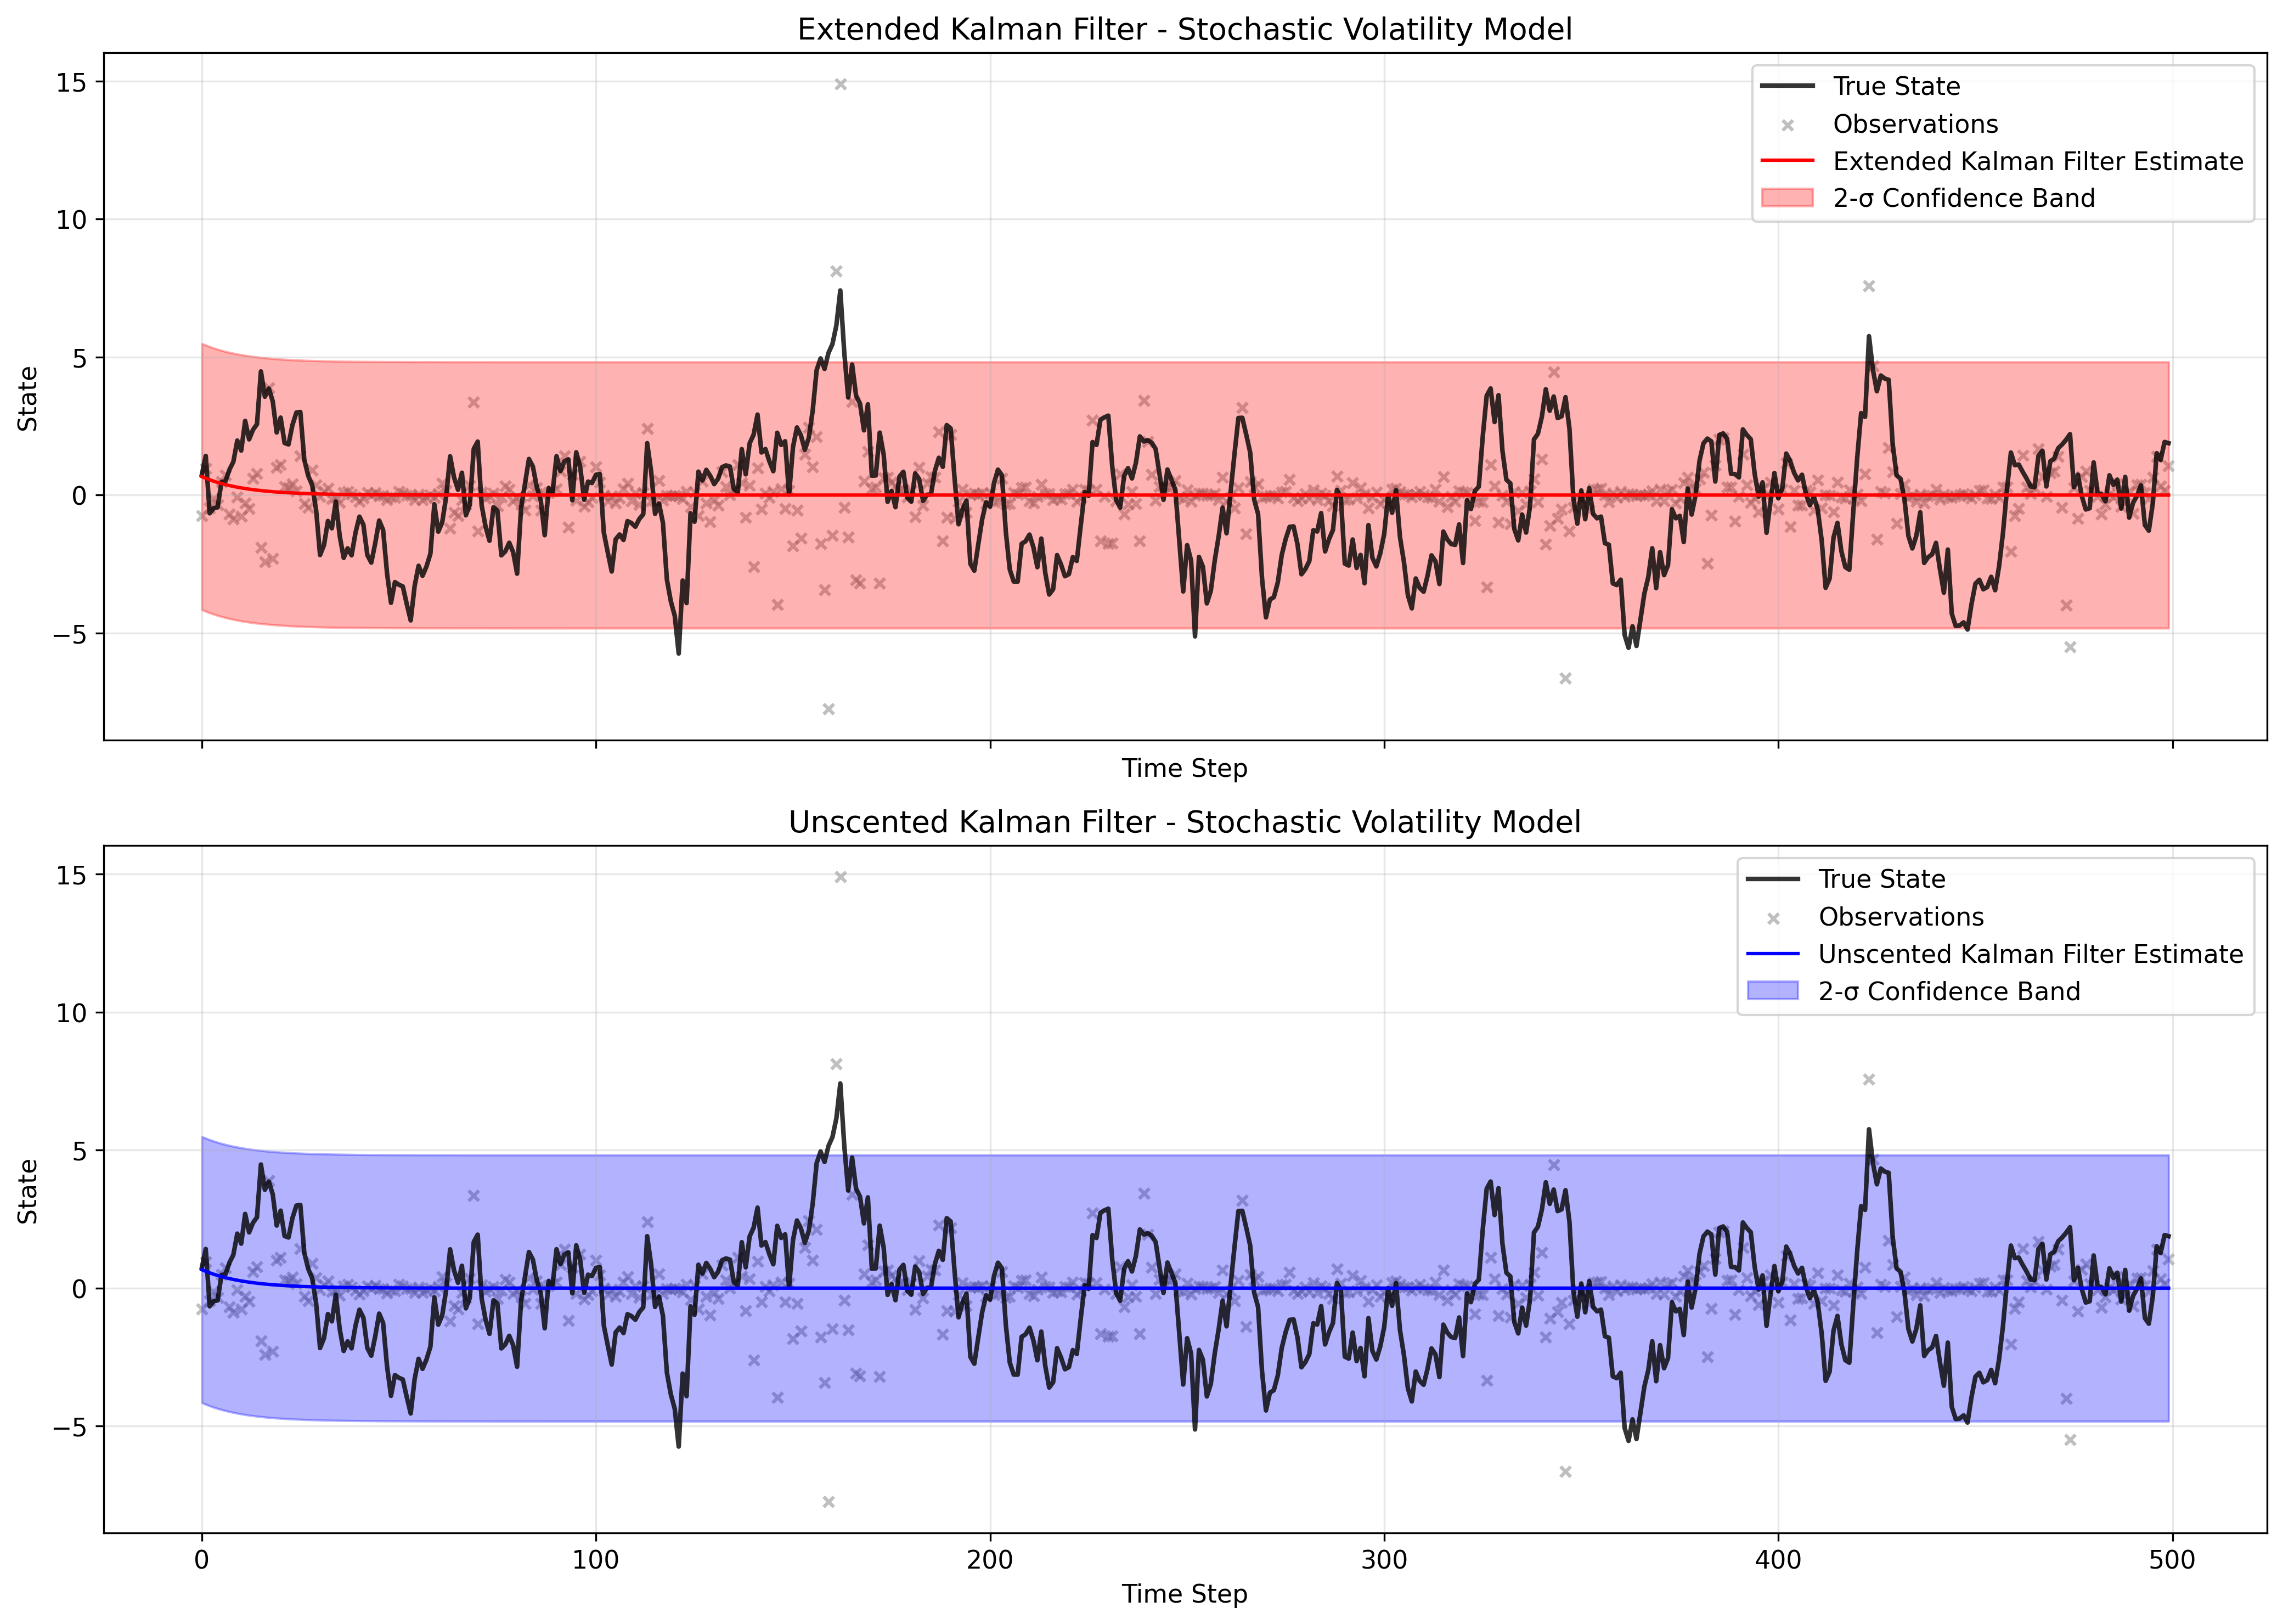
\includegraphics[width=0.8\linewidth]{sto_uekf2.png}
    \caption{EKF and UKF result on stochastic volatility model}
\end{figure}
\begin{figure}[H]
    \centering
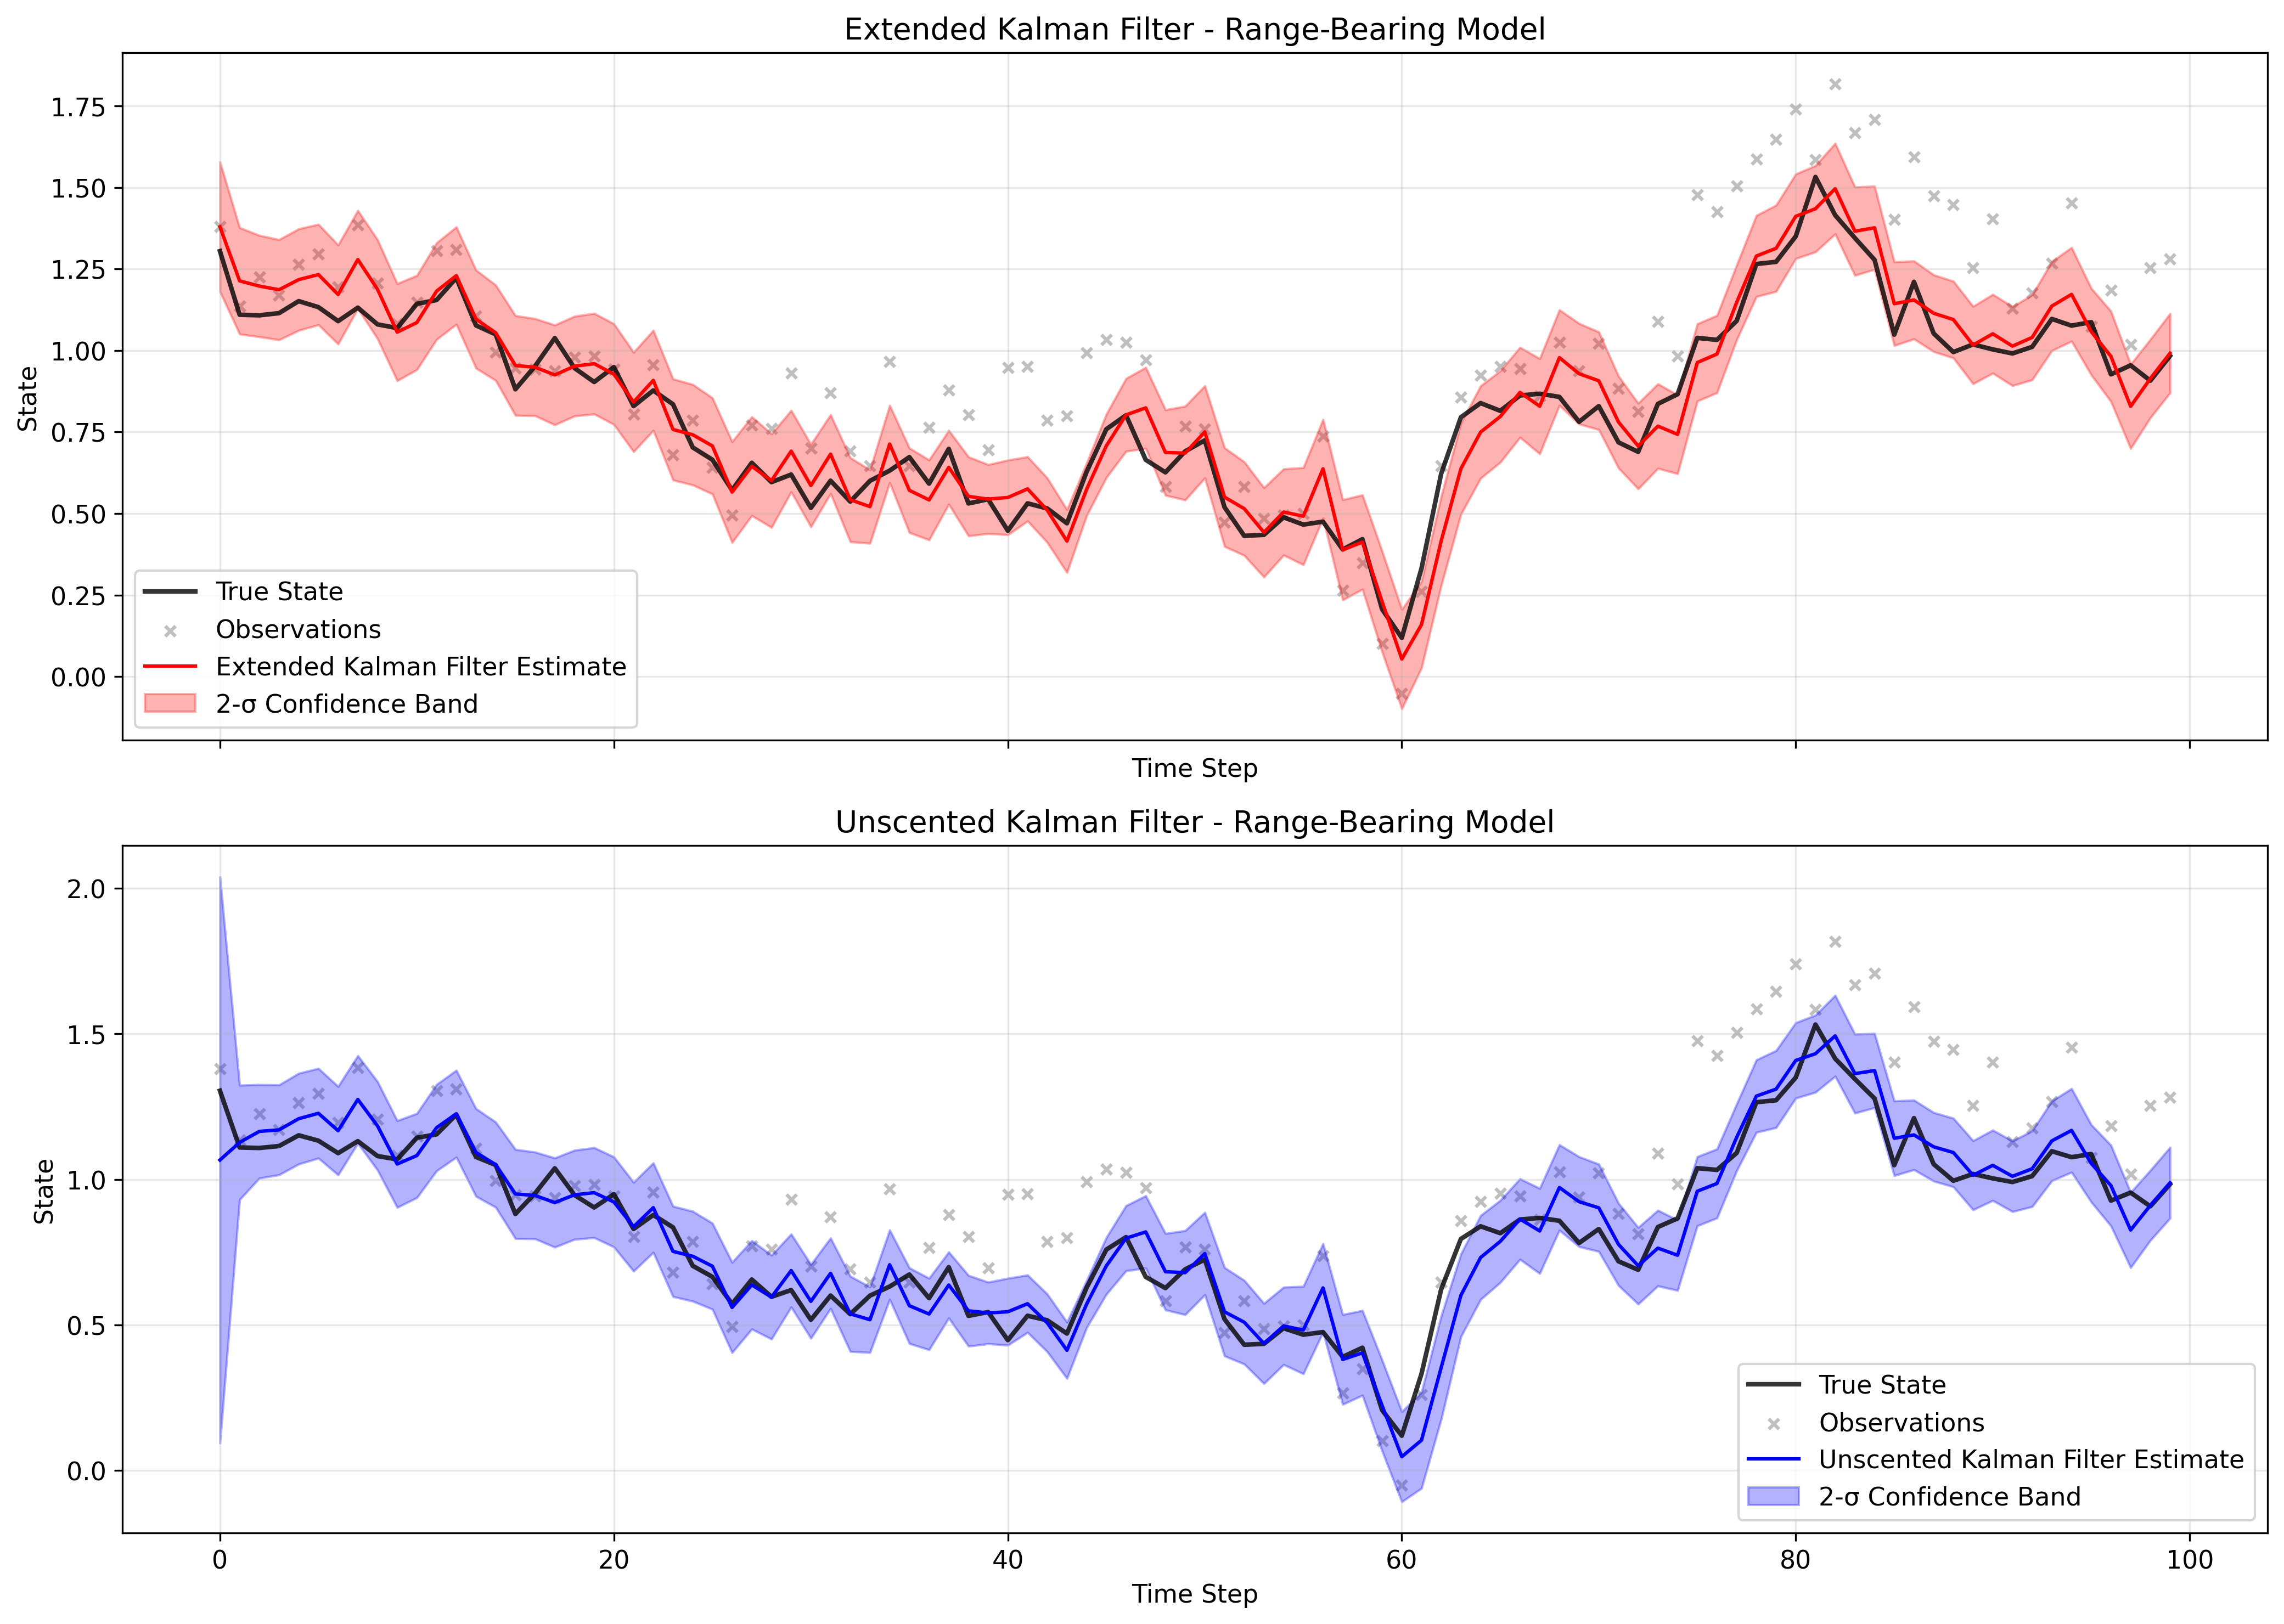
\includegraphics[width=0.8\linewidth]{rb_uekf.png}
    \caption{EKF and UKF result on range bearing model}
\end{figure}
we see that the range-bearing model works with UKF and EKF because we can get a reasonable Jacobian from the observation model.






\subsubsection{Particle Filter and Particle Degeneracy}


\begin{figure}[H]
    \centering
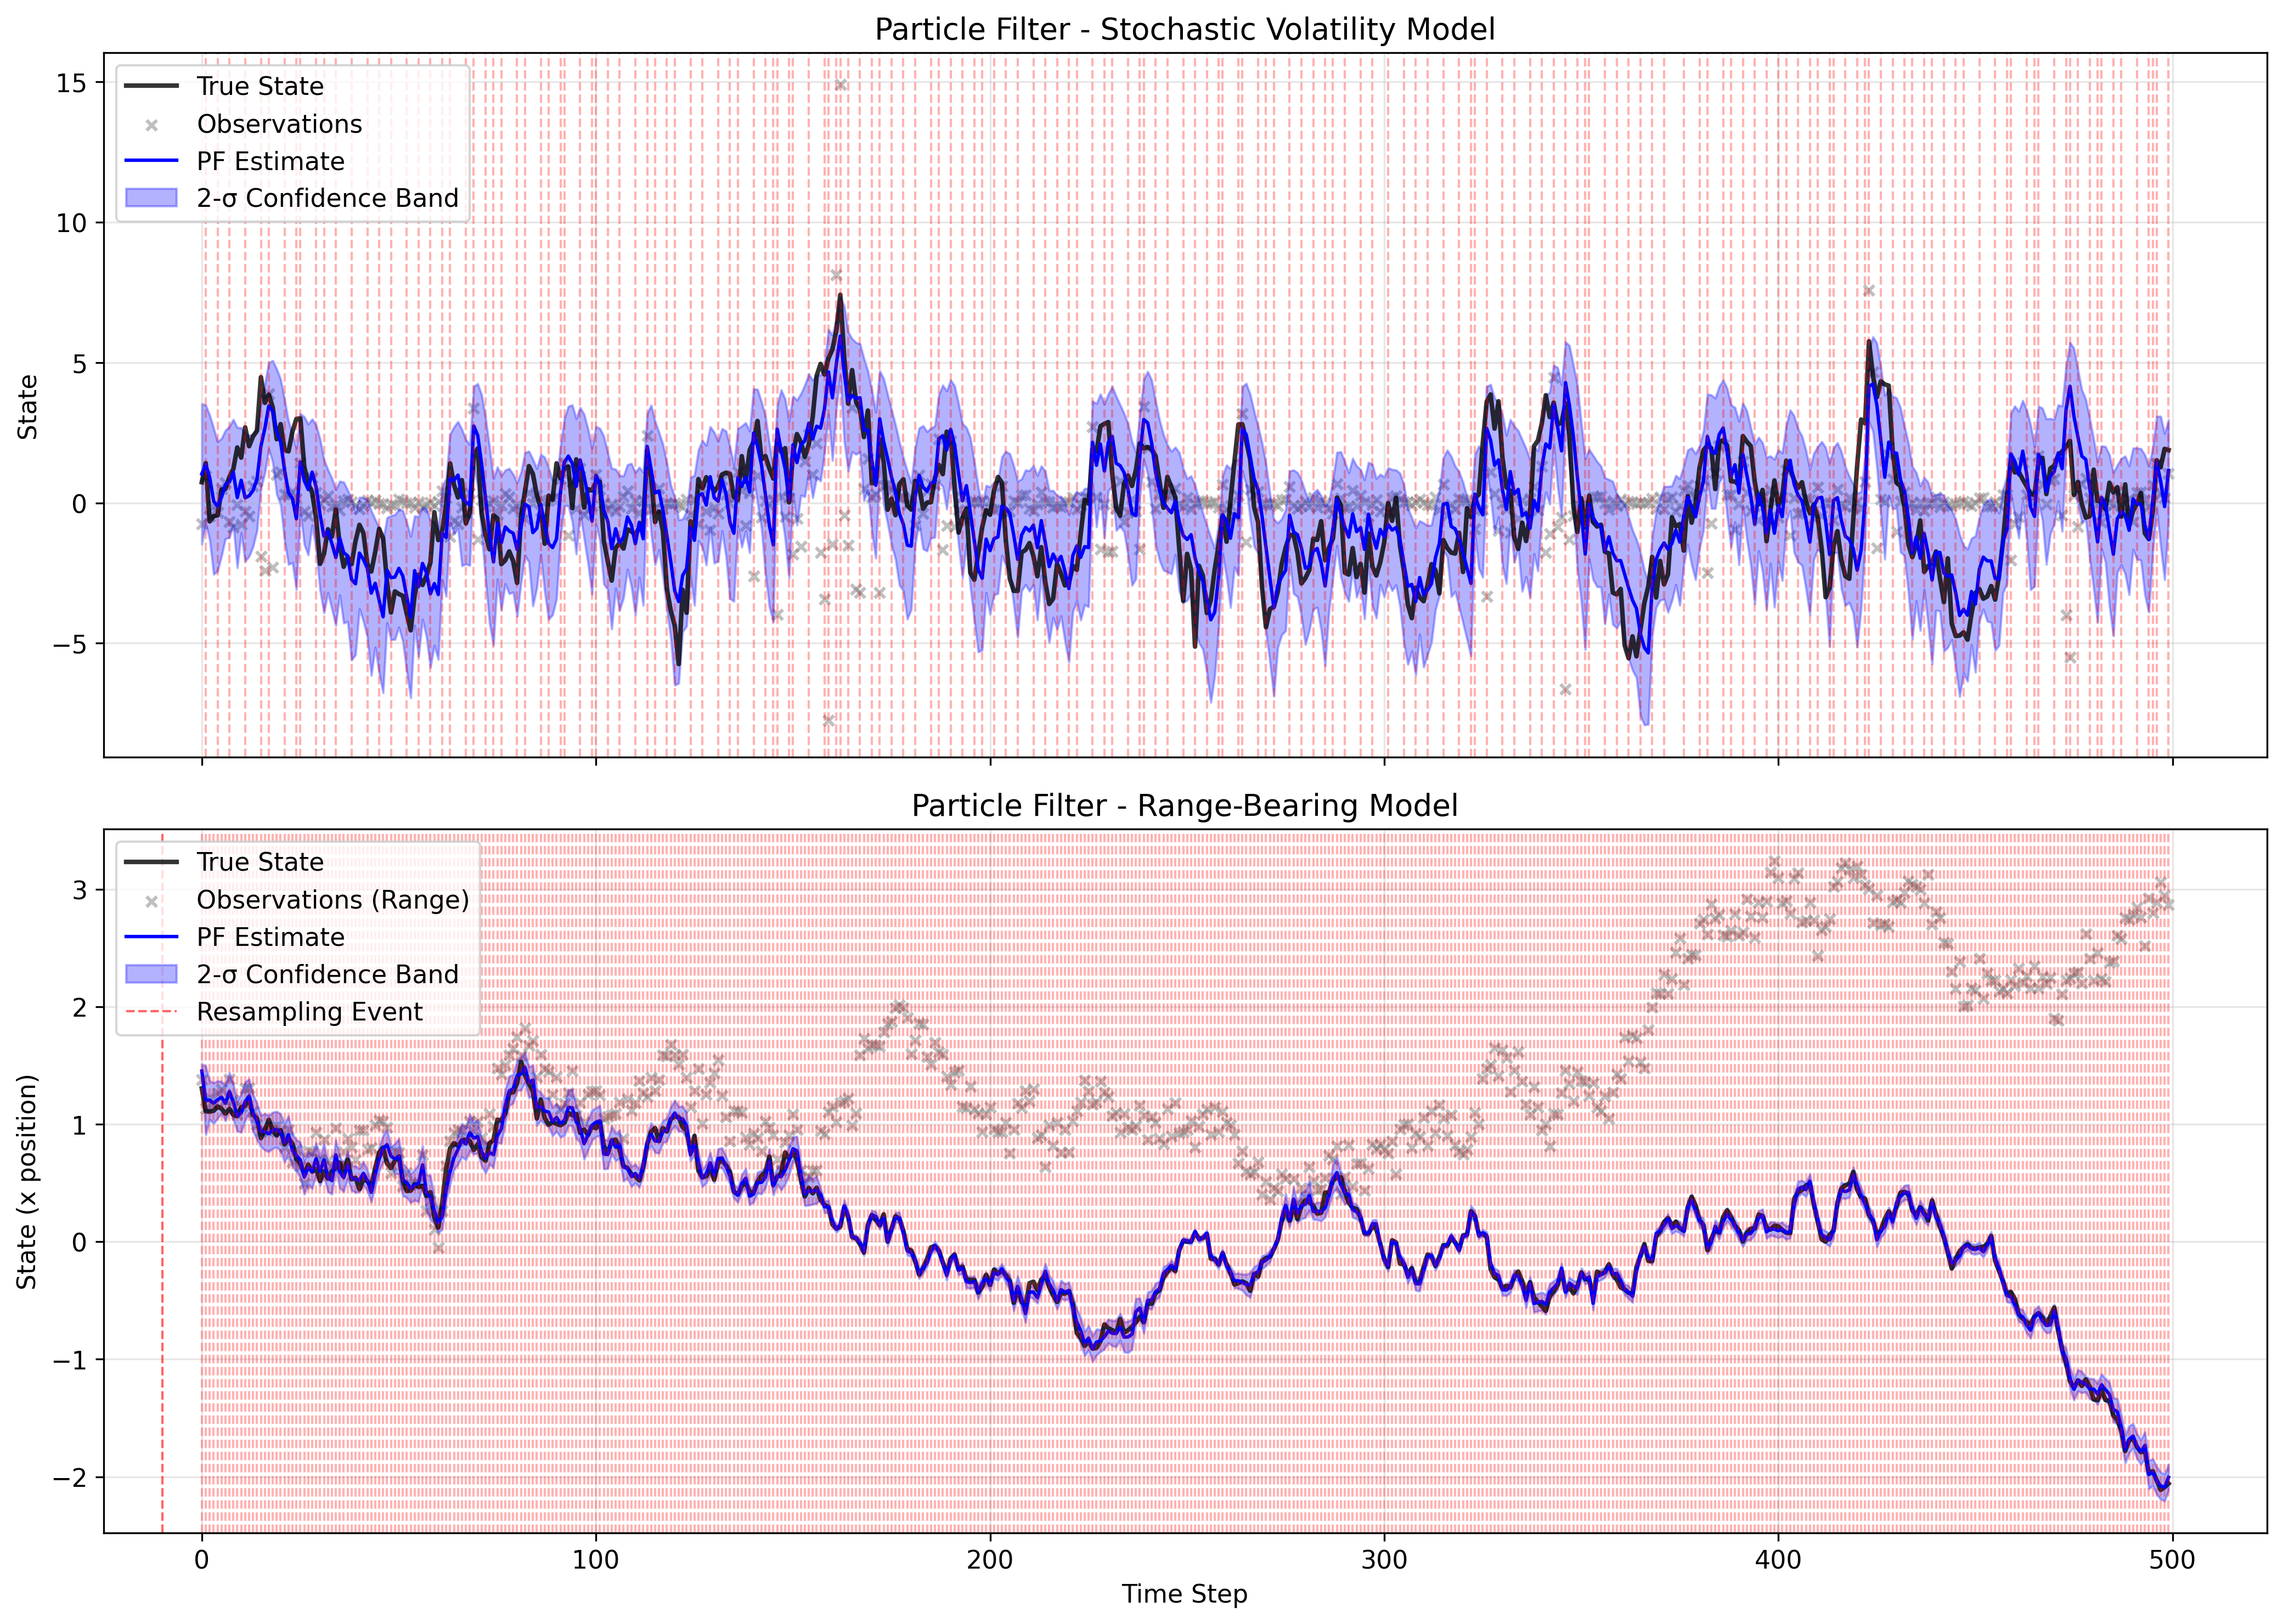
\includegraphics[width=0.8\linewidth]{particle.png}
    \caption{We see that particle filter tracking the means of both models pretty well}
    \label{fig:placeholder}
\end{figure}


\begin{figure}[H]
    \centering
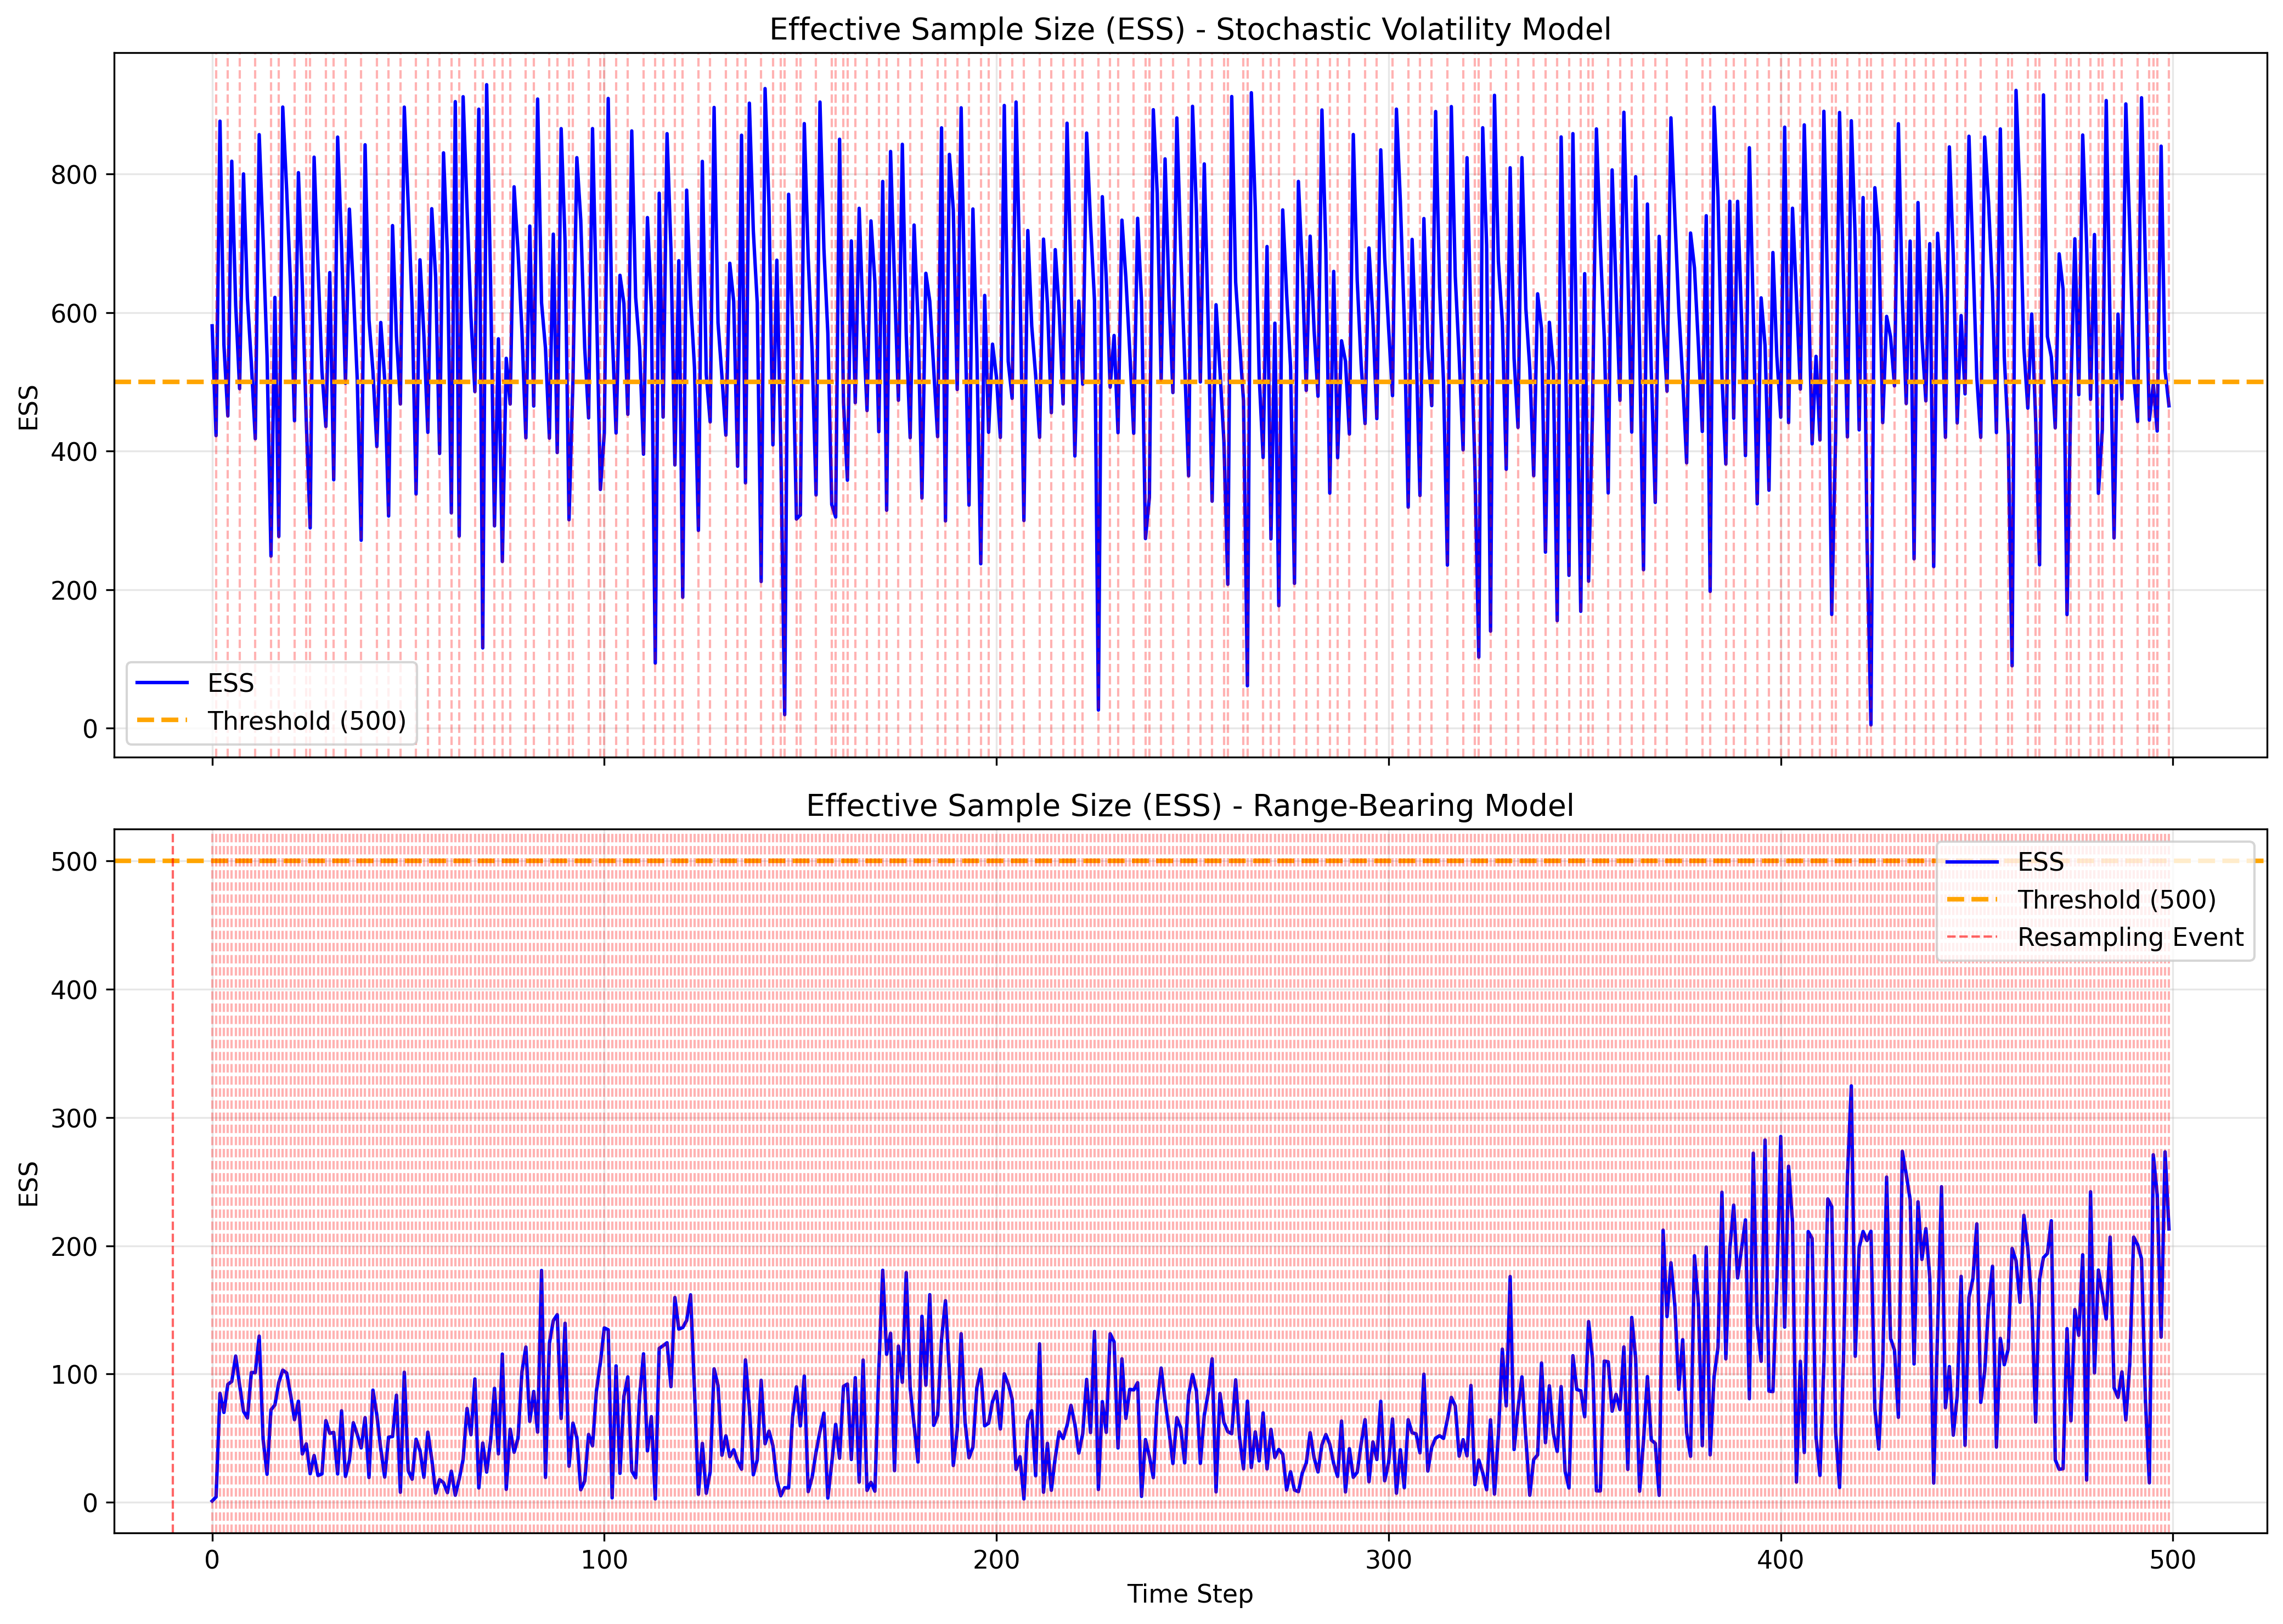
\includegraphics[width=0.8\linewidth]{particle2.png}
    \caption{Effective sample size a function of time}
    \label{fig:placeholder}
\end{figure}
The red lines are the times where we did resampling. It turns out that the range-bearing model had very bad initialization, but the particle filter somehow managed to increase sample size at later times. This is likely due to the fact that particles were moved into the right position, so even with very few particles, it can track the distribution very well. However, a depleted sample size means that uncertainty estimation is unreliable. 

\begin{figure}[H]
    \centering
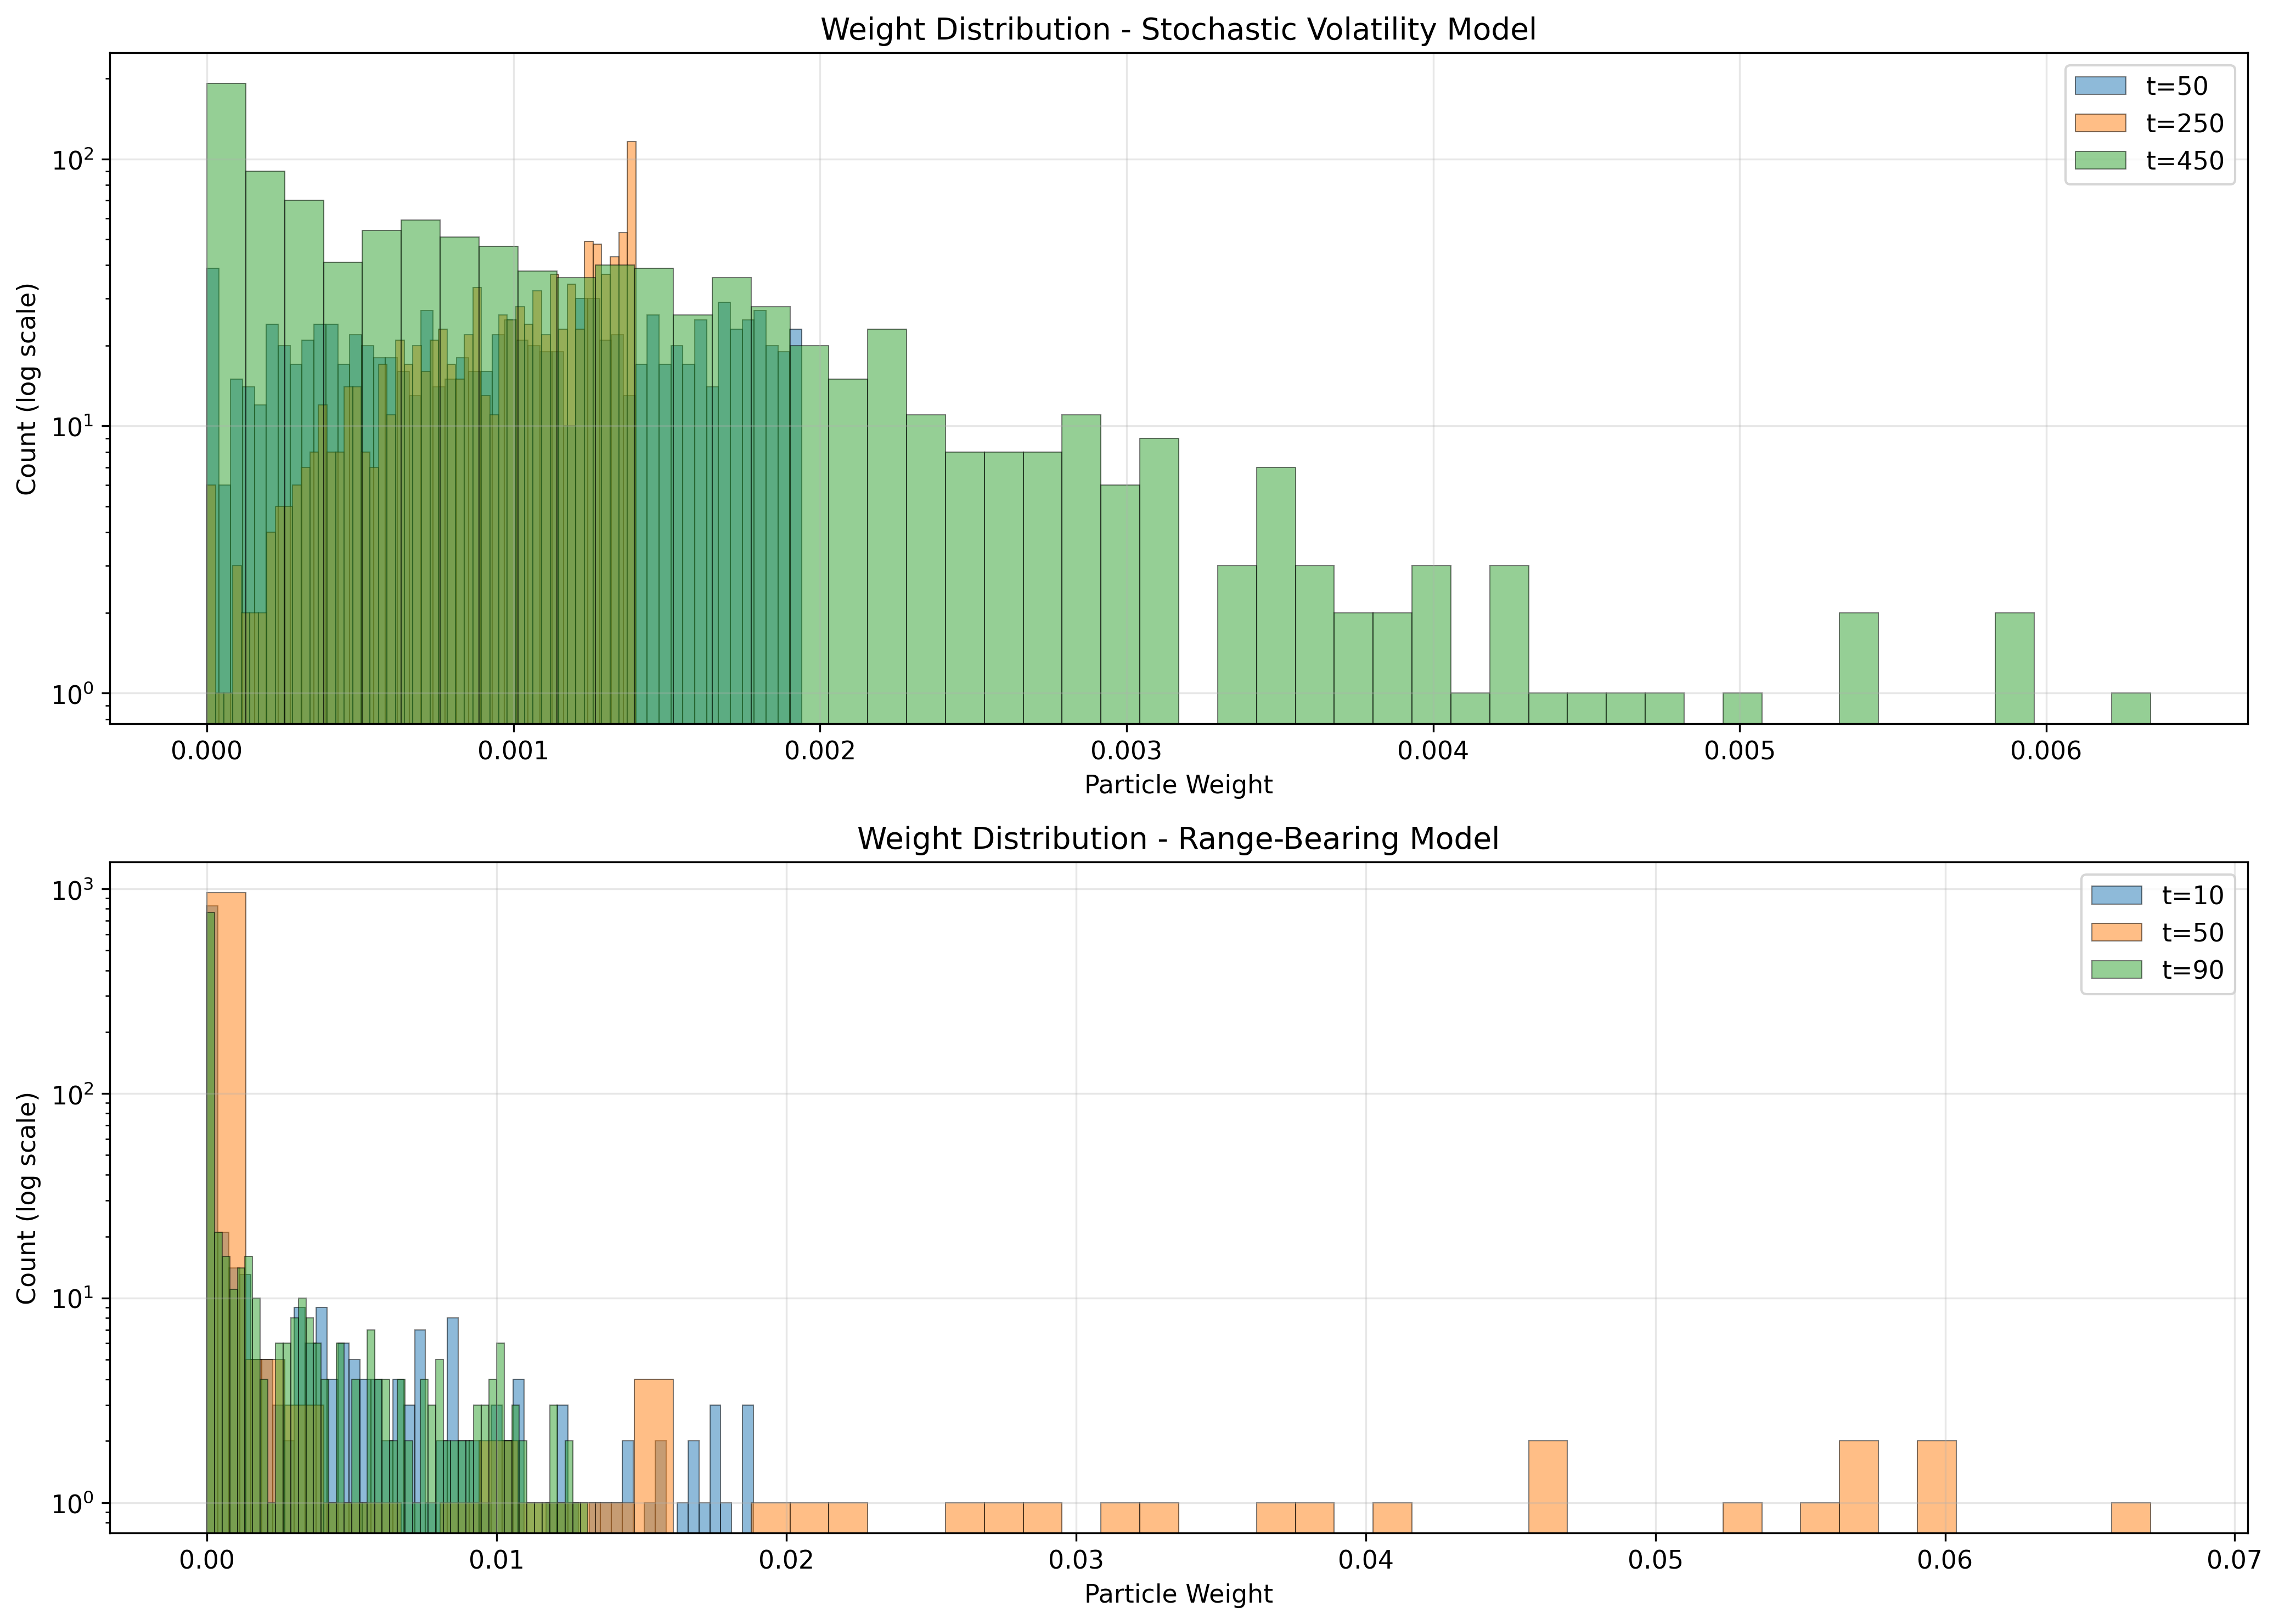
\includegraphics[width=0.8\linewidth]{particle3.png}
    \caption{Weight distribution at three different times. It further demonstrates that bad initialization for the range-bearing model had collapsed weight distribution from the very beginning}
    \label{fig:placeholder}
\end{figure}


\begin{figure}[H]
    \centering
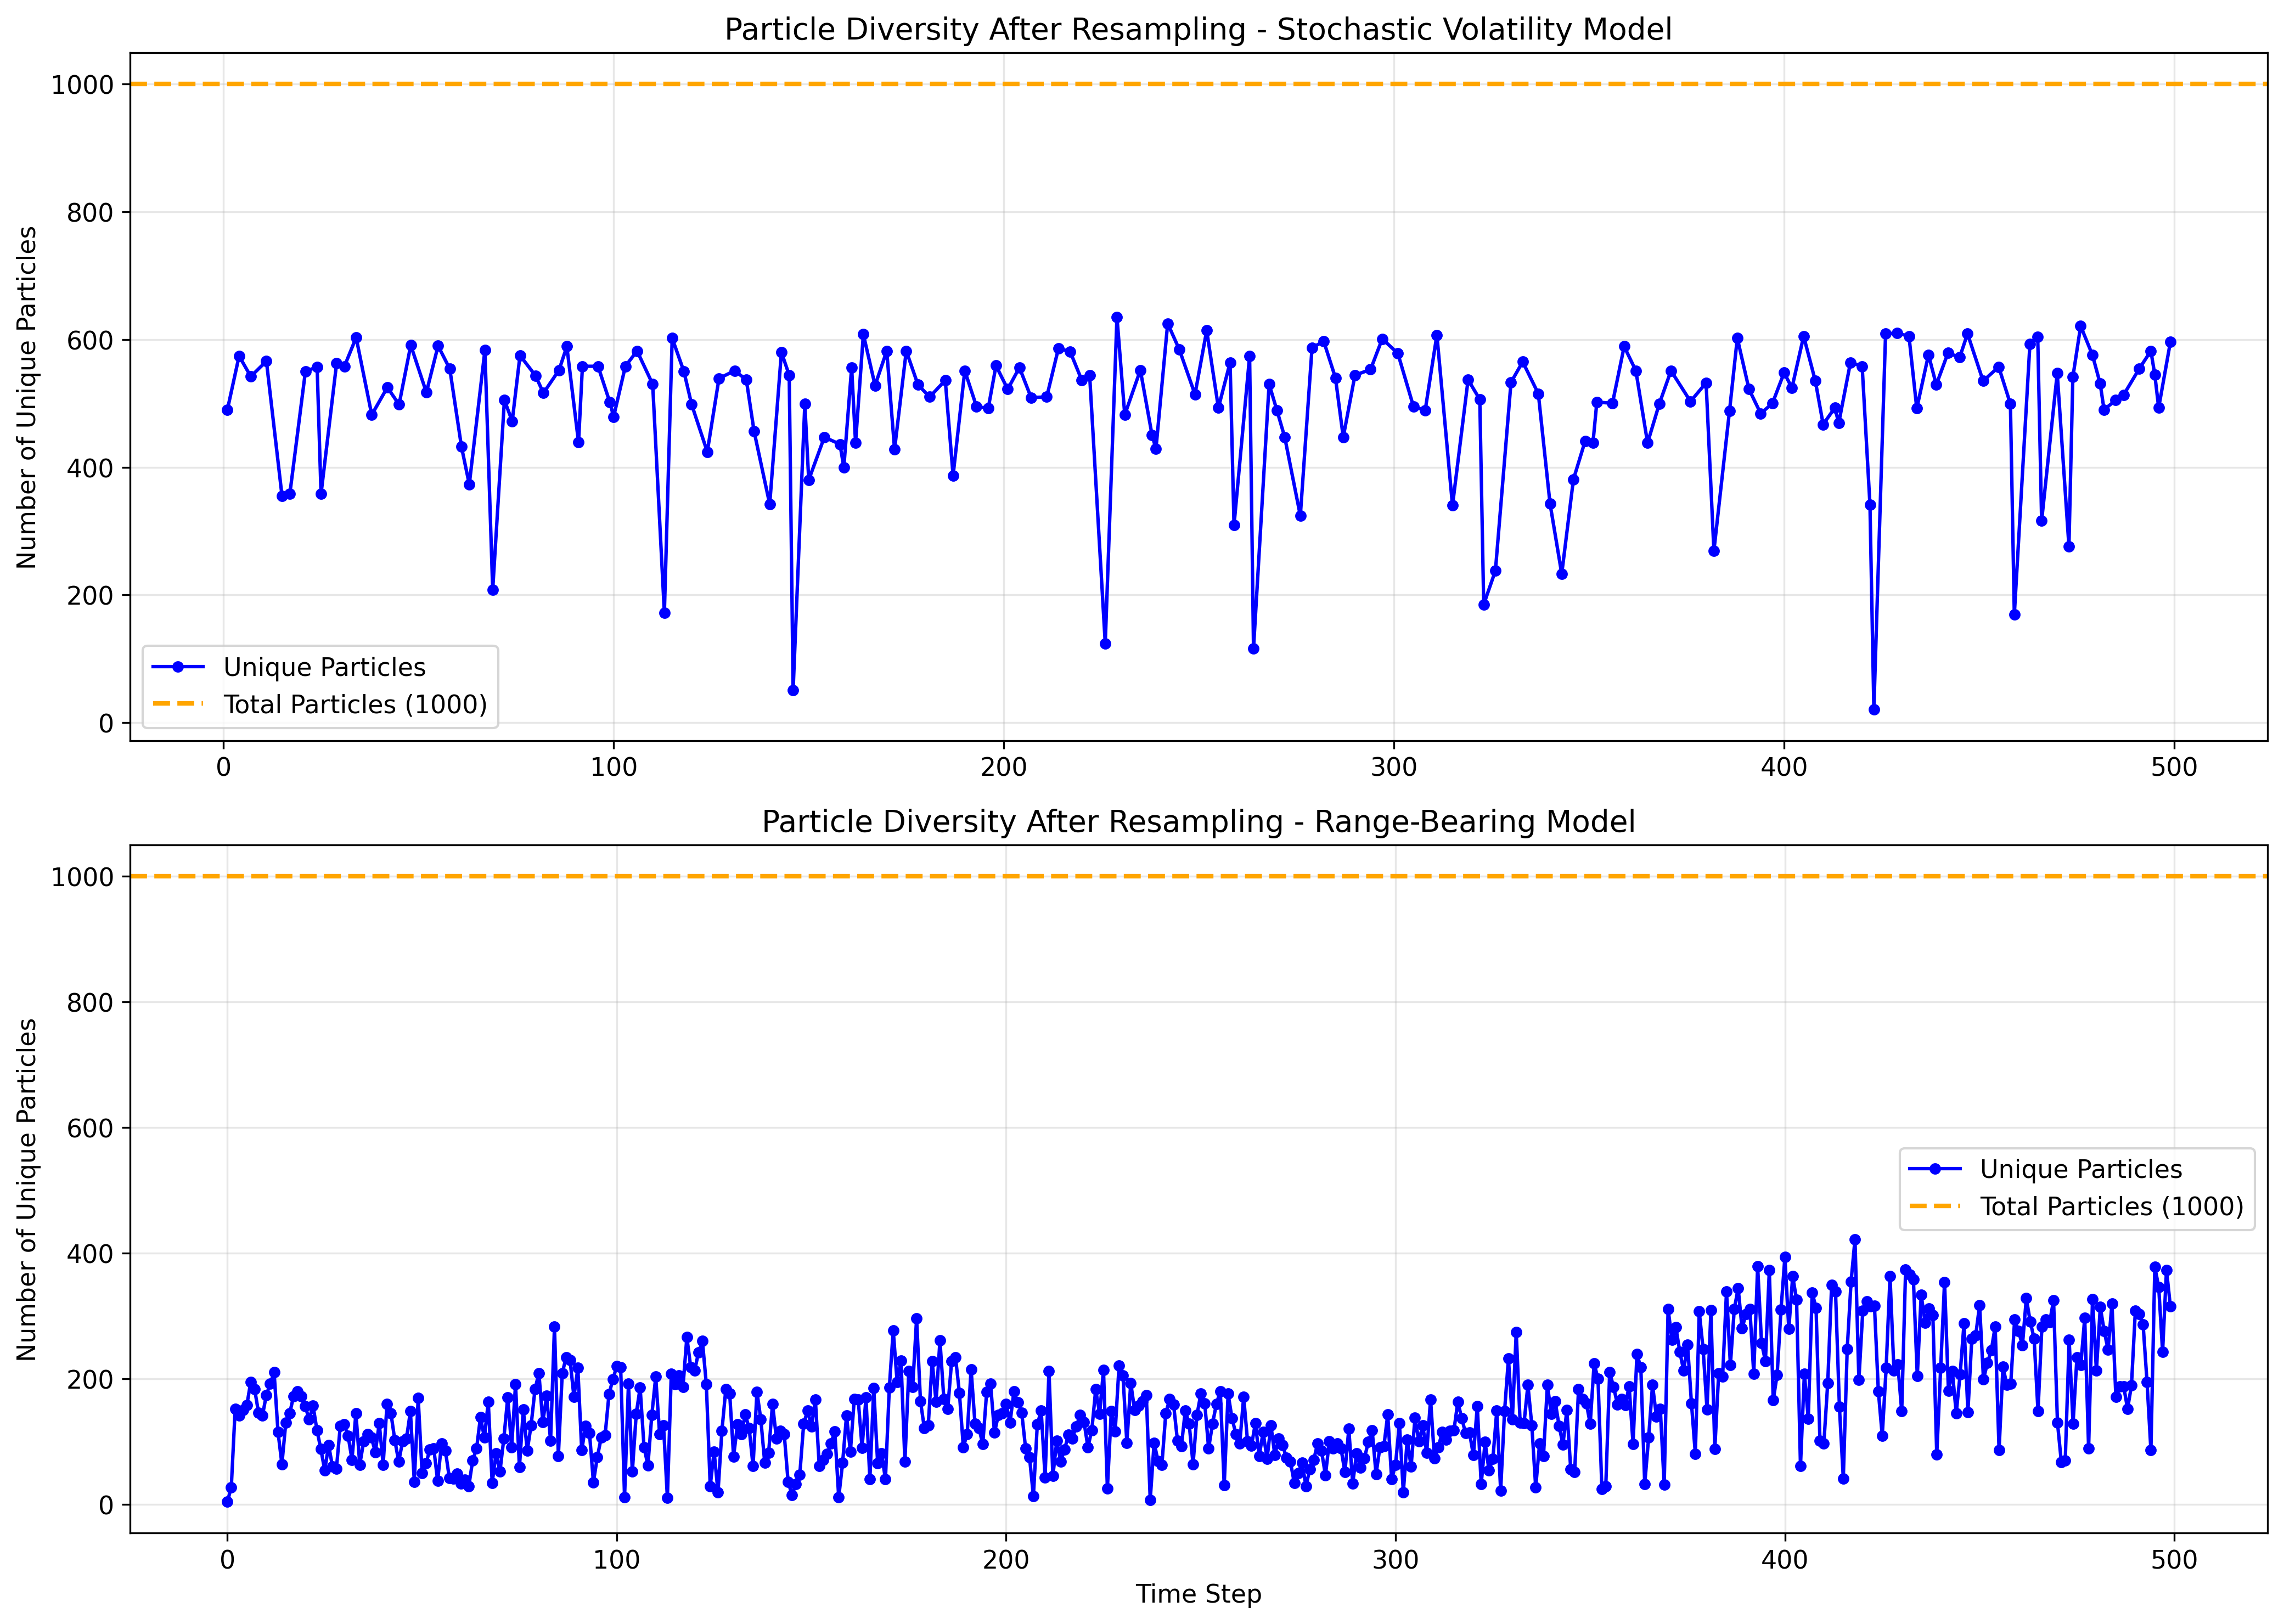
\includegraphics[width=0.8\linewidth]{particle4.png}
    \caption{Particle diversity for the Stochastic Volatility model is reasonable.  }
    \label{fig:placeholder}
\end{figure}

\subsubsection{EDH (LEDH) Flow and Filter}
My flow filter and invertible flow particle filter did not work for the acoustic tracking model or even the simplified acoustic tracking model. I could not reproduce the result from \cite{Li-Particle-Filtering-2017}. However, it works for the range-bearing model, so I include the performance for the range-bearing model here. It is similar to Table 1 from \cite{Li-Particle-Filtering-2017}. The performance of PF is the baseline, and all the flow and invertible filters outperform the Bootstrap particle filter. In addition, LEDH invertible has the best performance in terms of accuracy, but it is the slowest among all the filters.






\begin{table}[H]
\centering
\caption{Particle Filter Comparison on Range-Bearing Model}
\begin{tabular}{lccccc}
\toprule
\textbf{Filter} & \textbf{RMSE} & \textbf{Log-Lik} & \textbf{Wall Time (s)} & \textbf{Time/Step (ms)} & \textbf{Peak Mem (MB)} \\
\midrule
PF                & 0.0610 & 745.41  & 50.81  & 101.63  & 16.05  \\
EDH Flow          & 0.0593 & ---     & 7.26   & 72.55   & 1.48   \\
EDH Invertible    & 0.0584 & 423.50  & 22.15  & 221.48  & 4.64   \\
LEDH Flow         & 0.0584 & ---     & 228.09 & 2280.95 & 1.46   \\
LEDH Invertible   & 0.0582 & 428.97  & 163.06 & 1630.56 & 1.67   \\
\bottomrule
\end{tabular}
\\[1em]
\begin{tabular}{lccc}
\toprule
\textbf{Filter} & \textbf{Particles} & \textbf{Resample Rate} & \textbf{Timesteps} \\
\midrule
PF                & 1000 & 1.00 & 500 \\
EDH Flow          & 500  & ---  & 100 \\
EDH Invertible    & 2000 & 0.45 & 100 \\
LEDH Flow         & 500  & ---  & 100 \\
LEDH Invertible   & 500  & 0.37 & 100 \\
\bottomrule
\end{tabular}
\label{tab:range_bearing_comparison}
\end{table}



\subsubsection{Matrix Kernel Preventing Collapse}
\begin{figure}[H]
    \centering
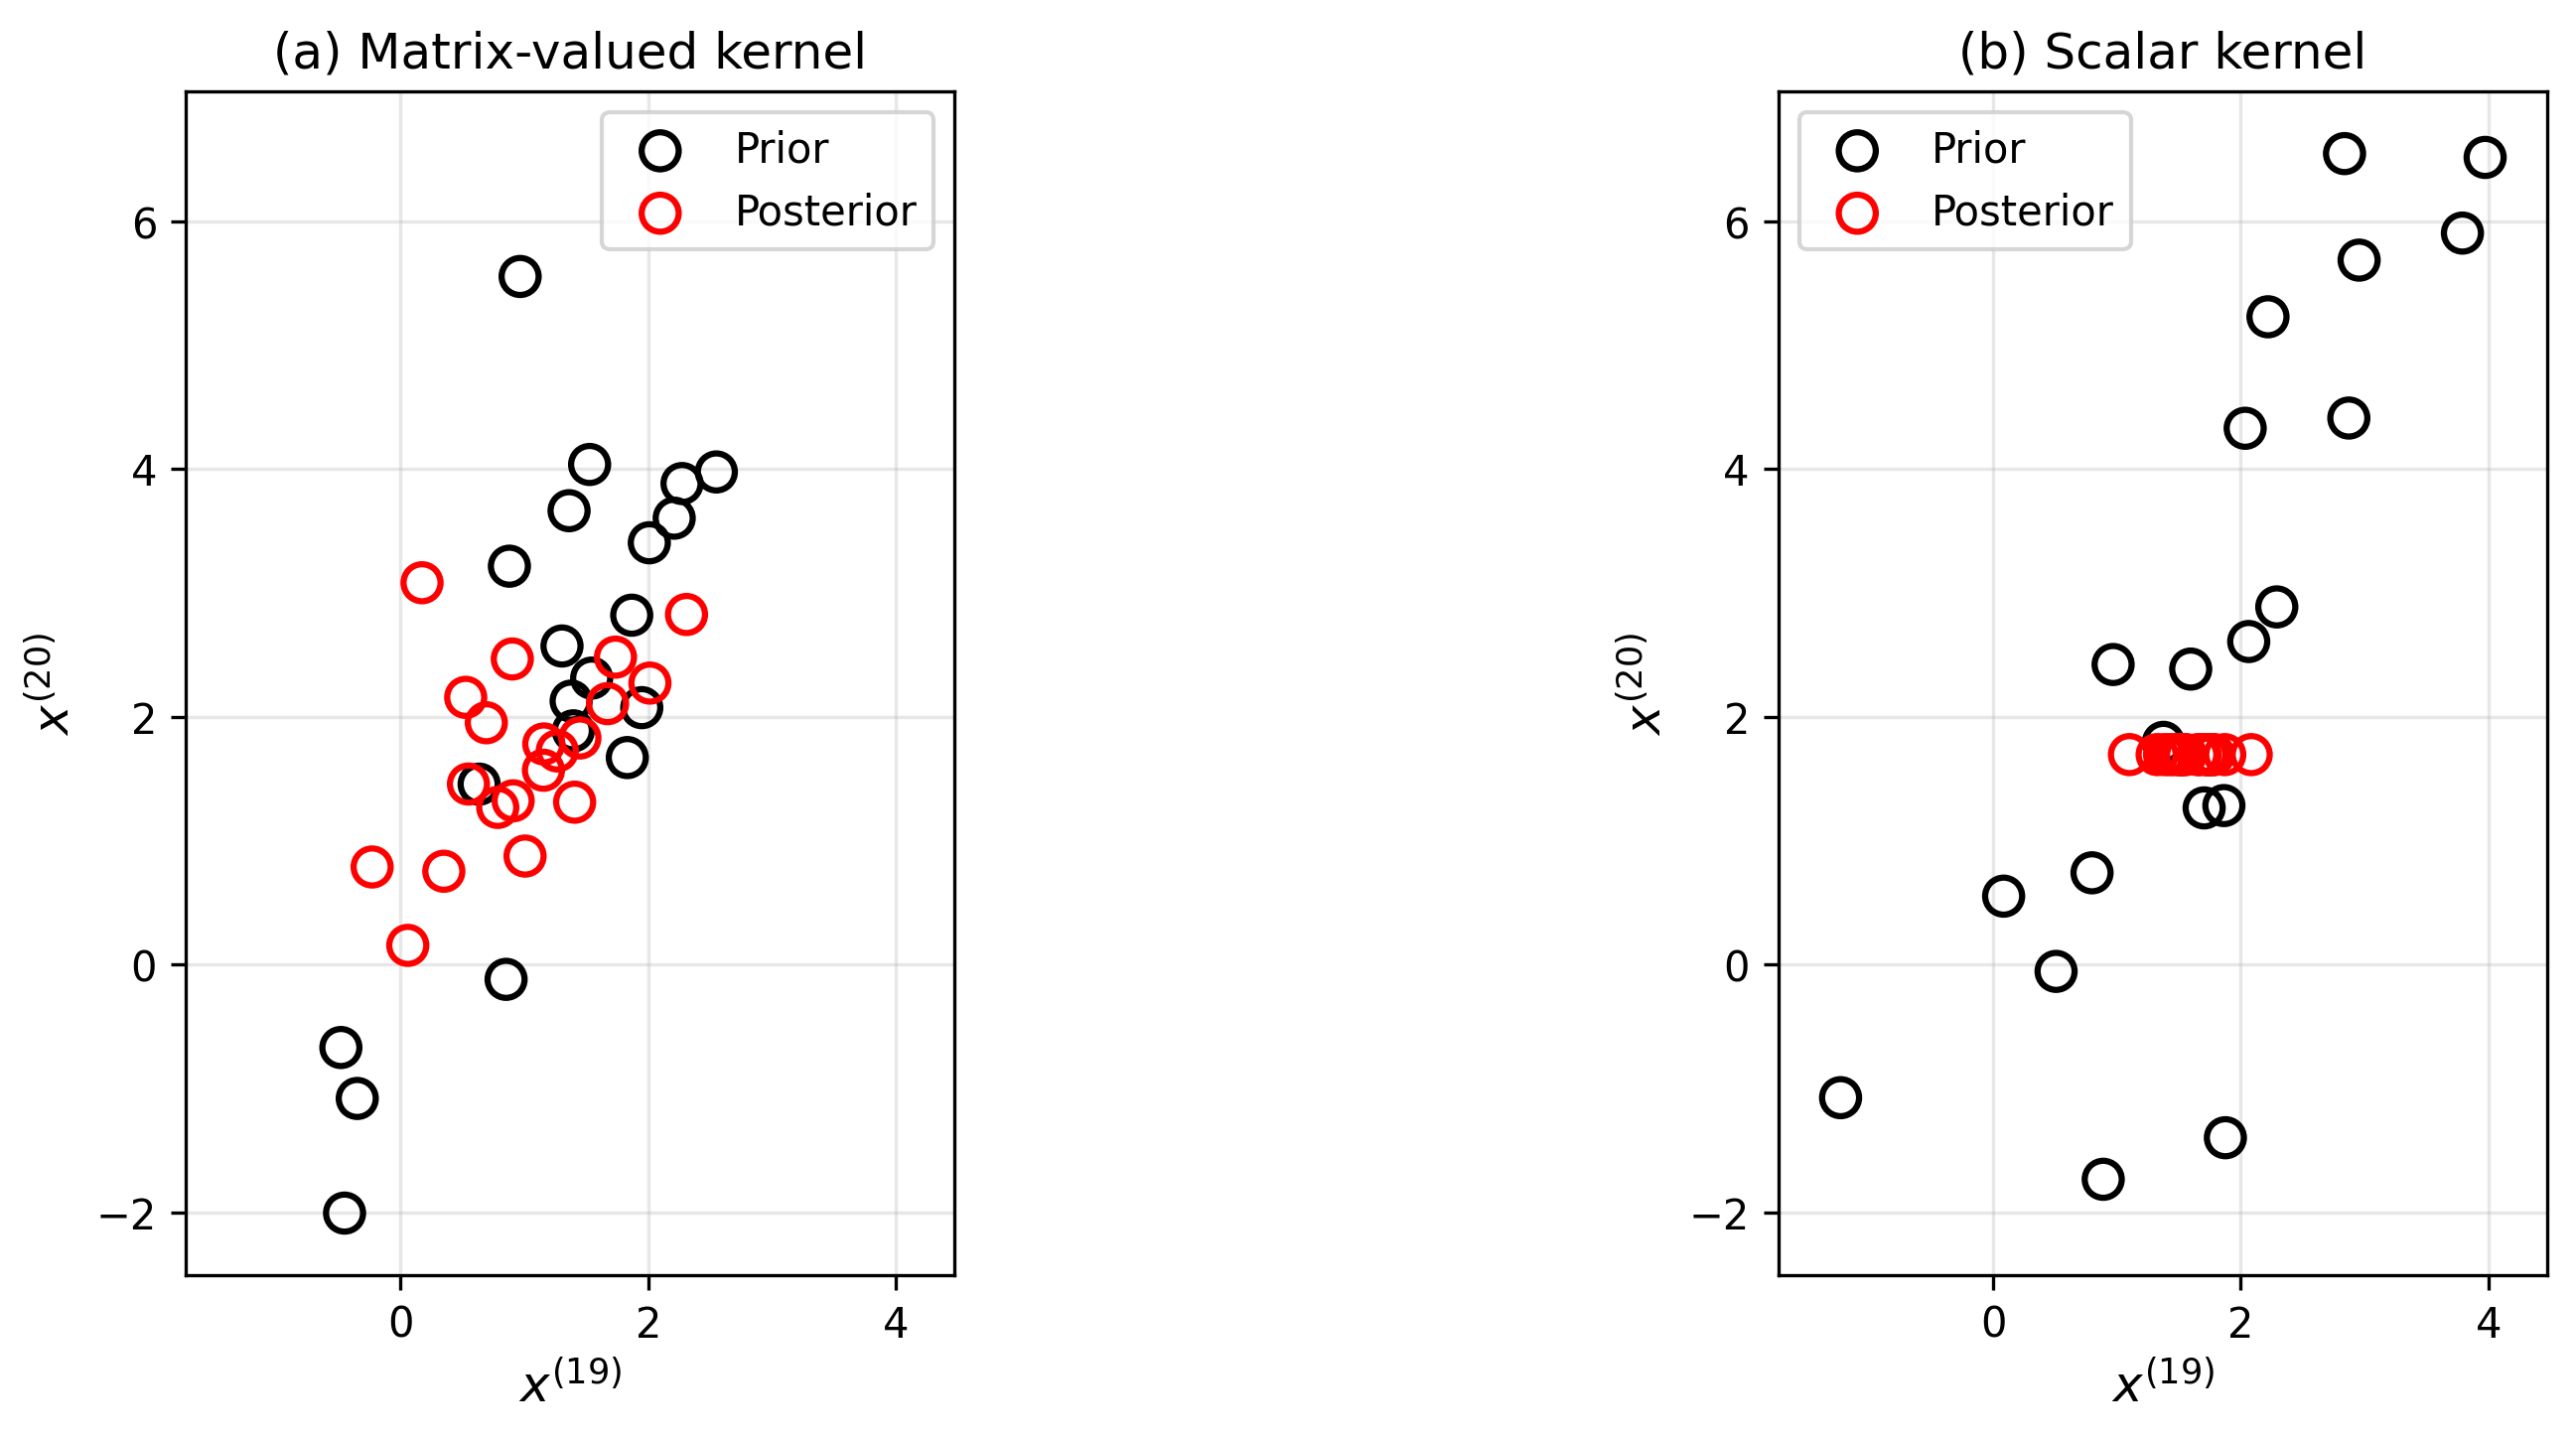
\includegraphics[width=0.5\linewidth]{figure3_reproduction.png}
    \caption{We can see clearly that by switching to a matrix kernel, $x_{20}$ no longer collapses into one point}
    \label{fig:placeholder}
\end{figure}
\newpage
\subsection{Part II}
\subsubsection{Stochastic Flow}

My stochastic flow filter is not working well even for the Kalman filter, and I have not yet been able to find out what is going on. It only works when the noise is set to zero. 
\begin{figure}[H]
    \centering
    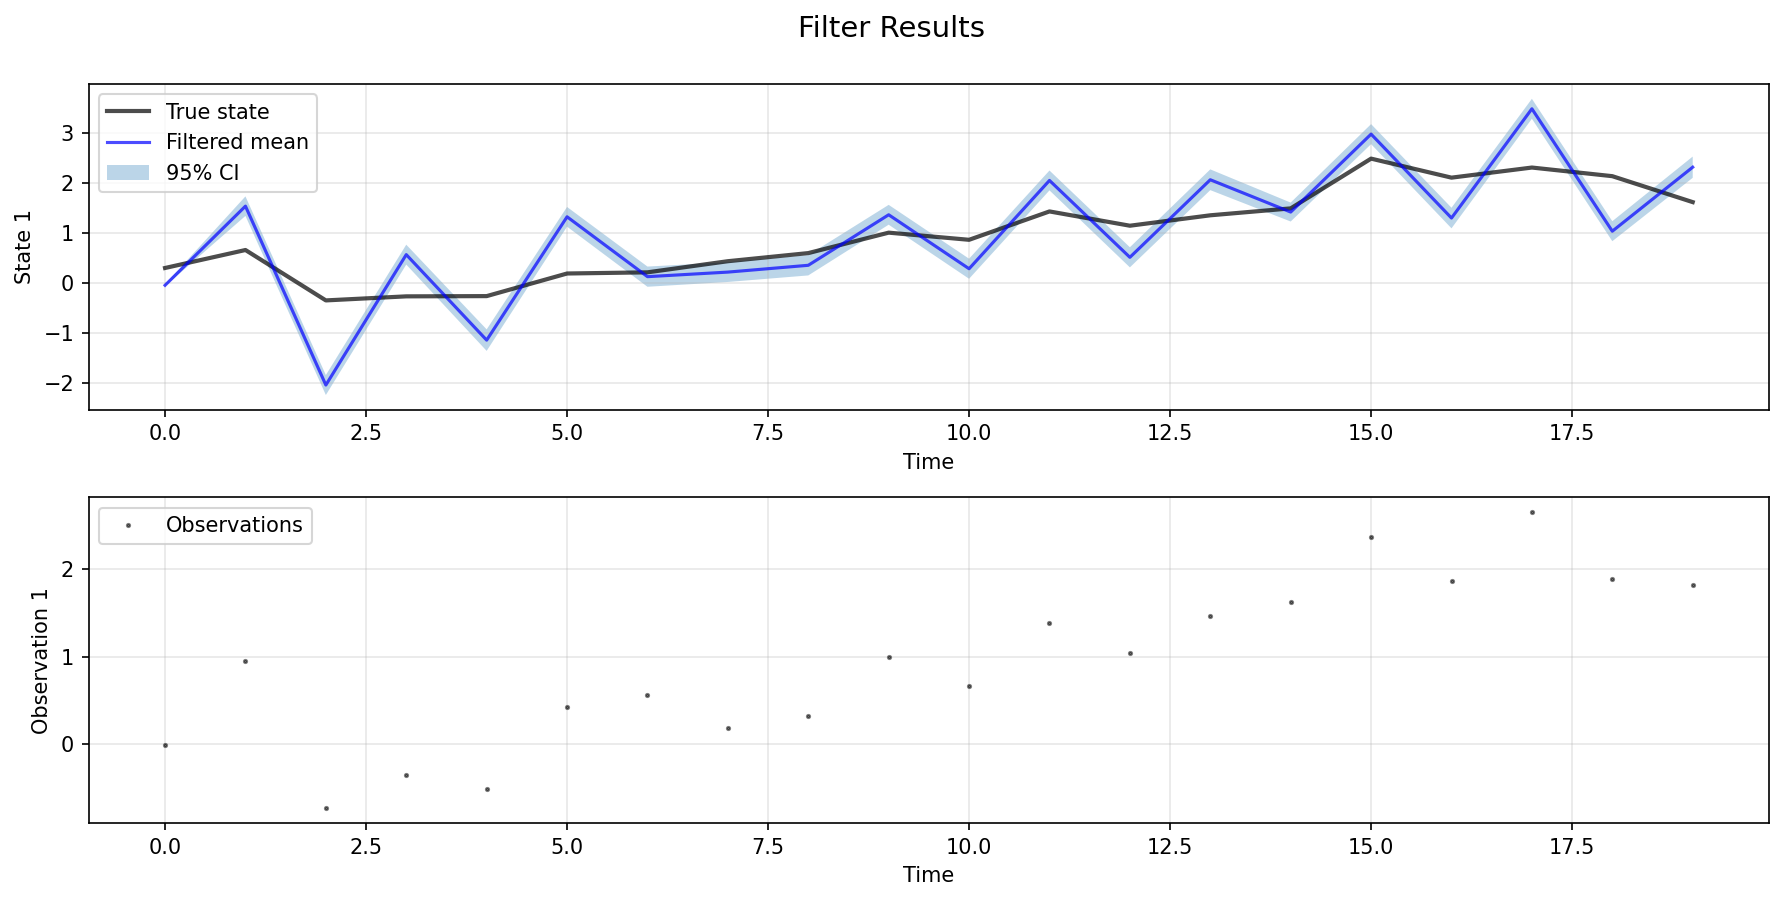
\includegraphics[width=0.5\linewidth]{sde_kalman.png}
    \caption{The current version of SDE filter, when diffusion scale is set to $0.001$}
    \label{fig:placeholder}
\end{figure}





\subsubsection{Soft Resampling and OT Resampling}

\begin{table}[htbp]
\centering
\caption{Resampling Method Comparison on Stochastic Volatility Model}
\begin{tabular}{lcccccc}
\toprule
\textbf{Method} & \textbf{Param} & \textbf{RMSE} & \textbf{Log-Lik} & \textbf{Wall Time (s)} & \textbf{Time/Step (ms)} & \textbf{Resample Rate} \\
\midrule
\multicolumn{7}{l}{\textit{Baseline}} \\
PF (Systematic) & ---    & 1.182 & $-436.29$ & 3.65  & 7.31  & 0.356 \\
\midrule
\multicolumn{7}{l}{\textit{Optimal Transport (OT) Resampling}} \\
OT              & $\epsilon=0.1$ & NaN   & NaN       & 32.61 & 65.23 & 0.290 \\
OT              & $\epsilon=0.3$ & 1.372 & $-477.29$ & 25.04 & 50.08 & 0.390 \\
OT              & $\epsilon=0.5$ & 1.379 & $-476.44$ & 18.32 & 36.65 & 0.390 \\
OT              & $\epsilon=1.0$ & NaN   & NaN       & 5.92  & 11.85 & 0.286 \\
\midrule
\multicolumn{7}{l}{\textit{Soft Resampling}} \\
Soft            & $\alpha=0.5$   & 1.173 & $-436.42$ & 1.26  & 2.52  & 0.534 \\
Soft            & $\alpha=0.7$   & 1.167 & $-436.04$ & 1.25  & 2.51  & 0.420 \\
Soft            & $\alpha=0.9$   & 1.175 & $-435.56$ & 1.27  & 2.54  & 0.368 \\
\bottomrule
\end{tabular}
\label{tab:stochastic_volatility_resampling}
\end{table}
Here I only have the results at their face value, so I will not speculate why the results turned out this way. 



\newpage
\section{A Few Words of Reflection}
This is a well-structured test, and I learned a lot from doing the background research, especially the knowledge I gained about Optimal Transport, which might actually turn out to be useful in the future. I now intend to learn about other applications of filtering and experiment with them more.

I didn't completely finish the test. I only included the experiments that directly relate to the question, even though I ran quite a few others. I simply ran out of time to write up the results properly.
I appreciate the experience. It made me realize that I need to manage my time better when navigating multiple commitments. I put too much focus on reading background material and exploring ideas for using neural networks to improve filtering. In the end, I didn't have enough time left to debug the code, complete the experiments, or write tests that would actually catch numerical instability. During my academic years, I never had to write formal tests for my code, so this was by far the biggest challenge I've faced. My original plan was to first make things work, then go back and add tests to check the edge cases. Maybe that approach just doesn't work well when I'm adding tests after the fact.
I will continue working on this project and force myself to write proper tests to debug the invertible flow code. Right now, I still cannot reproduce the results from \cite{Li-Particle-Filtering-2017}, because the acoustic tracking model breaks all of my EDH flow, EDH invertible, and their local counterparts.

Thank you for giving me this opportunity to do the test!


\newpage
\appendix
\section{Kalman Family}\label{APP:Kalman}
\textbf{Notation:}
\\
\begin{itemize}
\item $\v m^-_{t}$= \textit{a priori} state estimate (mean of the predicted distribution)
\item $\v m_t$= \textit{a posteriori} state estimate (mean of the updated distribution)
\item $\v P^-_t$ = \textit{a priori} error covariance
\item $\v P_t$ = \textit{a posteriori} error covariance
\item $p(x_k|z_{1:k-1})$=  prior distribution 
\item $p(x_k | z_{1:k})$ =  posterior Distribution
\end{itemize}
we use the following initial condition,
\begin{equation}
p(x_0) = \mathcal{N}(x_0 | m_0, P_0)
\end{equation}

For the Kalman filter, the noise and operators are both Gaussian, so the distributions stay Gaussian at all times. All we need to do is to keep track of the mean and variance of the prior distribution $p(x_k | y_{1:k})$. In the predict step, the goal is to compute $p(x_t | z_{1:t-1})$ from $p(x_{t-1} | z_{1:t-1})$.
Given $p(x_{t-1} | z_{1:t-1}) = \mathcal{N}(x_{t-1} | m_{t-1}, P_{t-1})$, we have:
\begin{equation}
p(x_t | z_{1:t-1}) = \int dx_{t-1} \, p(x_t | x_{t-1}) \, p(x_{t-1} | z_{1:t-1})
\end{equation}
From the state evolution model:
\begin{equation}
p(x_t | x_{t-1}) = \mathcal{N}(x_t | f x_{t-1}, Q)
\end{equation}
predicted/evolved mean is,
\begin{align}
m_t^- &= \mathbb{E}[x_t | z_{1:t-1}] \\
&= f m_{t-1}
\end{align}
predicted/evolved variance
\begin{align}
P_t^- &= \text{Var}[x_t | y_{1:t-1}] \\
&= Q + f^2 P_{t-1}
\end{align}
from the predict step, we get,
\begin{equation}
p(x_t | z_{1:t-1}) = \mathcal{N}(x_t | m_t^-, P_t^-)
\end{equation}
where
\begin{equation}
\boxed{m_t^- = a m_{t-1}, \quad P_t^- = a^2 P_{t-1} + Q}
\end{equation}
In the update step, we need to incorporate observation $z_t$ using Bayes' rule.
\begin{equation}
p(x_t | z_{1:t}) = \frac{p(z_t | x_t) \, p(x_t | z_{1:t-1})}{p(z_t | z_{1:t-1})}
\end{equation}
From the observation model:
\begin{equation}
p(z_t | x_t) = \mathcal{N}(z_t | h x_t, R)
\end{equation}
We need to compute the product of two Gaussians:
\begin{align}
p(x_t | z_{1:t}) &\propto \mathcal{N}(z_t | h x_t, R) \cdot \mathcal{N}(x_t | m_t^-, P_t^-) \\
&\propto \exp\left(-\frac{1}{2}\frac{(z_t - h x_t)^2}{R}\right) \exp\left(-\frac{1}{2}\frac{(x_t - m_t^-)^2}{P_t^-}\right)
\end{align}

Expanding the exponents:
\begin{align}
-\frac{1}{2}\left[\frac{(z_t - h x_t)^2}{R} + \frac{(x_t - m_t^-)^2}{P_t^-}\right] &= -\frac{1}{2}\left[\frac{z_t^2 - 2 z_t h x_t + h^2 x_t^2}{R} + \frac{x_t^2 - 2 x_t m_t^- + (m_t^-)^2}{P_t^-}\right]
\end{align}
Collecting terms in $x_t^2$ and $x_t$: $-\frac{1}{2}\left[\left(\frac{h^2}{R} + \frac{1}{P_t^-}\right) x_t^2 - 2\left(\frac{h z_t}{R} + \frac{m_t^-}{P_t^-}\right) x_t + \text{const}\right]$.
This is a Gaussian in $x_t$. Completing the square, we have $\frac{1}{P_t} = \frac{h^2}{R} + \frac{1}{P_t^-}$. $P$ is the uncertainty, so the inverse of $P$ is like precision; by adding information about the measurement $\frac{h^2}{R}$, we get additional precision, which is exactly what we are aiming for. When $\frac{h^2}{R}=0$, namely large noise from observation, we say we can't trust the measurement and we should stick with the dynamics. We see that both mean and variance will receive no update. On the other hand, if $\frac{h^2}{R} \ll \frac{1}{P_t^-}$, then the observation will carry more weight and the result from dynamics should be disregarded.
The updated variance is
\begin{align}
P_t = \frac{R P_t^-}{h^2 P_t^- + R}
\end{align}
For simplicity, we define the \textbf{Kalman gain:}
\begin{equation}
K_t = \frac{P_t^- h}{h^2 P_t^- + R}
\end{equation}
Then:
\begin{equation}
P_t = (1 - K_t h) P_t^-
\end{equation}
After some algebra:
\begin{equation}
m_t = m_t^- + K_t (z_t - h m_t^-)
\end{equation}
where we denote the innovation $v_t=z_t-hm^-$, namely the difference between the real observation and the predicted observation from prior mean.
In summary, we get,
\begin{equation}
\boxed{
\begin{aligned}
K_t &= \frac{P_t^- h}{h^2 P_t^- + R} \\
v_t &= y_t - h m_t^-
m_t &= m_t^- + K_t v_t \\
P_t &= (1 - K_t h) P_t^-
\end{aligned}
}
\end{equation}
At this point, we can already see that what the filter does is to correct the distribution based on the observed data point. Essentially, we want the mean and covariance from the updated distribution at each time step. For higher dimensions, all we have to do is to promote the scalar recursive relation into matrices.  
\textbf{Prediction Step:}
\begin{align}
\hat{\v{x}}_t^- &= \v{\hat F} \hat{\v{x}}_{t-1}^+ \\
\v{P}_t^- &= \v{\hat F} \v{P}_{t-1}^+ \v{\hat F}^T + \v{Q}
\end{align}
\textbf{Correction Step:}
\begin{align}
\v{\hat K}_t &= \v{P}_t^- \v{H}^T \left[\v{H} \v{P}_t^- \v{H}^T + \v{R}\right]^{-1} \quad \text{(Kalman gain)} \\
\hat{\v{x}}_t^+ &= \hat{\v{x}}_t^- + \v{K}_t (\v{z}_t - \v{H}\hat{\v{x}}_t^-) \\
\v{\hat P}_t^+ &= (\v{I} - \v{K}_t \v{H}) \v{P}_t^-
\end{align}
We know that the Kalman filter requires linear models and Gaussian noise. However, this is very restrictive. For cases where the noises are Gaussian but models are non-linear, we have the Extended Kalman filter (EKF) and Unscented Kalman Filter (UKF). The idea for the extension is to somehow make approximations so that we can use the Kalman filter. EKF linearizes the models via first-order Taylor expansion around the current estimate.
\begin{equation}
\v{F}_t = \left.\frac{\partial f}{\partial \v{x}}\right|_{\v{x} = \hat{\v{x}}_{t-1}^+}, \quad
\v{H}_t = \left.\frac{\partial h}{\partial \v{x}}\right|_{\v{x} = \hat{\v{x}}_t^-}
\end{equation}
Apply Kalman filter equations using time-varying $\v{F}_t, \v{H}_t$. Evolve using time-dependent operators,
\begin{align}
\hat{\v{x}}_t^- &= f(\hat{\v{x}}_{t-1}^+) \\
\v{P}_t^- &= \v{F}_t \v{P}_{t-1}^+ \v{F}_t^T + \v{Q}
\end{align}
Update using  $\v{H}_t$ and predicted measurement $\hat{\v{z}}_t^- = h(\hat{\v{x}}_t^-)$.
\begin{align}
\v{\hat K}_t &= \v{P}_t^- \v{H}_t^T \left[\v{H}_t \v{P}_t^- \v{H}_t^T + \v{R}\right]^{-1} \quad \text{(Kalman gain)} \\
\hat{\v{x}}_t^+ &= \hat{\v{x}}_t^- + \v{K}_t (\v{z}_t - \v{H}_t\hat{\v{x}}_t^-) \\
\v{\hat P}_t^+ &= (\v{I} - \v{K}_t \v{H}_t) \v{P}_t^-
\end{align}

However, there are strong limitations to this approach, namely: only first-order accurate; can diverge for strong nonlinearity; requires Jacobian computation (may be expensive or analytically intractable); assumes Gaussian noises. As for the UKF, it propagates uncertainty through nonlinear functions using \textbf{sigma points} (also called unscented points) - deterministically chosen samples that capture mean and covariance. Here we further introduce some definitions:
\begin{itemize}
\item $\v P_{zz,t}^{-}$ = predicted measurement covariance
\item $\v P_{xz,t}^{-}$ = cross-covariance between state and measurement
\end{itemize}
This is because Kalman gain has a more general form \begin{equation}
\v K_t = \v P_{xz,t}^{-} \bigl( \v P_{zz,t}^{-} \bigr)^{-1}
\label{eq:general-kalman-gain}
\end{equation}

where
\begin{itemize}
\item $\v P_{xz,t}^{-} = \Cov(\v x_t - \hat{\v x}_t^{-}, \v z_t - \hat{\v z}_t^{-})$ \quad (state–innovation cross-covariance)
\item $\v P_{zz,t}^{-} = \Cov(\v z_t - \hat{\v z}_t^{-})$ \quad (innovation covariance)
\end{itemize}

This expression is exact for the linear-Gaussian case and approximate (but very effective) for nonlinear cases when the covariances are estimated via linearization (EKF) or sigma points (UKF). Associated with the sigma points are two sets of weights used for computing the mean and covariance after nonlinear transformation:

\begin{align}
W_0^{(m)} &= \frac{\lambda}{n + \lambda} \\
W_0^{(c)} &= \frac{\lambda}{n + \lambda} + (1 - \alpha^2 + \beta) \\
W_i^{(m)} &= W_i^{(c)} = \frac{1}{2(n + \lambda)}, \quad i = 1, \dots, 2n
\end{align}

where
\begin{itemize}
\item $W^{(m)}_i$ are used to recover the transformed \textbf{mean},
\item $W^{(c)}_i$ are used to recover the transformed \textbf{covariance},
\item $\beta$ is typically set to 2 (optimal for Gaussian distributions).
\item $\alpha$ - Spread Control Parameter, we set it to $10^{-3}$
\item $\kappa$  - Secondary Scaling Parameter, we set it to zero.
\item $\lambda = \alpha^2(n_x + \kappa) - n_x$
\end{itemize}












\textbf{Prediction Step (Time Update):}

Generate $2n_x + 1$ sigma points from $\hat{\v x}_{t-1}$ and $\v P_{t-1}$ (augmented form with process noise is common in literature, but here we show the standard non-augmented version for clarity and consistency with EKF notation):

\begin{align}
\v{\chi}_{t-1}^{(0)} &= \hat{\v x}_{t-1} \\
\v{\chi}_{t-1}^{(i)} &= \hat{\v x}_{t-1} + \bigl(\sqrt{(n_x + \lambda) \v P_{t-1}}\bigr)_i \quad i=1,\dots,n_x \\
\v{\chi}_{t-1}^{(i)} &= \hat{\v x}_{t-1} - \bigl(\sqrt{(n_x + \lambda) \v P_{t-1}}\bigr)_{i-n_x} \quad i=n_x+1,\dots,2n_x
\end{align}

Propagate through the nonlinear state transition:

\begin{equation}
\v{\chi}_{t|i}^{-} = f\bigl( \v{\chi}_{t-1}^{(i)} \bigr), \quad i=0,\dots,2n_x
\end{equation}

Compute predicted mean and covariance:

\begin{align}
\hat{\v x}_{t}^{-} &= \sum_{i=0}^{2n_x} W_i^{(m)} \, \v{\chi}_{t|i}^{-} \\
\v P_{t}^{-} &= \sum_{i=0}^{2n_x} W_i^{(c)} \, \bigl( \v{\chi}_{t|i}^{-} - \hat{\v x}_{t}^{-} \bigr) \bigl( \v{\chi}_{t|i}^{-} - \hat{\v x}_{t}^{-} \bigr)^\top
\end{align}

\textbf{Update Step (Measurement Update):}

Propagate sigma points through the nonlinear measurement function:

\begin{equation}
\v{\zeta}_{t|i}^{-} = h\bigl( \v{\chi}_{t|i}^{-} \bigr), \quad i=0,\dots,2n_x
\end{equation}

Compute predicted measurement mean, innovation covariance, and cross-covariance:

\begin{align}
\hat{\v z}_{t}^{-} &= \sum_{i=0}^{2n_x} W_i^{(m)} \, \v{\zeta}_{t|i}^{-} \\
\v P_{zz,t}^{-} &= \sum_{i=0}^{2n_x} W_i^{(c)} \, \bigl( \v{\zeta}_{t|i}^{-} - \hat{\v z}_{t}^{-} \bigr) \bigl( \v{\zeta}_{t|i}^{-} - \hat{\v z}_{t}^{-} \bigr)^\top \\
\v P_{xz,t}^{-} &= \sum_{i=0}^{2n_x} W_i^{(c)} \, \bigl( \v{\chi}_{t|i}^{-} - \hat{\v x}_{t}^{-} \bigr) \bigl( \v{\zeta}_{t|i}^{-} - \hat{\v z}_{t}^{-} \bigr)^\top
\end{align}

Define the \textbf{innovation}:

\begin{equation}
\v v_t = \v z_t - \hat{\v z}_{t}^{-}
\end{equation}

Compute the \textbf{Kalman gain}:

\begin{equation}
\v K_t = \v P_{xz,t}^{-} \bigl( \v P_{zz,t}^{-} \bigr)^{-1}
\end{equation}

Update state mean and covariance:

\begin{align}
\hat{\v x}_{t} &= \hat{\v x}_{t}^{-} + \v K_t \, \v v_t \\
\v P_{t} &= \v P_{t}^{-} - \v K_t \, \v P_{zz,t}^{-} \, \v K_t^\top
\end{align}



\newpage 

\section{Particle flow and particle filter}


\subsection{Particle flow}

Previously, we have discussed how after each resampling, the information of the distribution is concentrated on the multiplicity distribution of the particles, and the diversity of the particles has been lost. If we look at the particle methods, it's clear that we either use weights or multiplicity distribution to mimic the distribution. The culprit of the particle degeneracy is the consecutive multiplication of small numbers: $p(y_t | x_t^{(i)})$ will make a large number of particles irrelevant after a few steps. The observation was done independently and there is no way to control the value of $p(y_t | x_t^{(i)})$. In \cite{daum2010exact,daum2011particle}, the author proposed using the multiplicity to store the information of the distribution and invented an alternative evolution for the particles such that $p(y_t | x_t^{(i)})$ was never too small. The limitation of these two papers is that to solve the equation, which we will talk about later, they have to assume a linear or nearly linear observation model and dynamics with additive Gaussian noise. The evolution for the particles is a completely different equation than the underlying dynamics for the ground truth. Later, we will see methods that generalize the equation for more general noise distributions. Let us first derive the evolution equations. First, we have the prediction step: 
\begin{align}
p(x_t | z_{1:t-1})=g(x_t)
\end{align}
and the "observation" step,
\begin{align}
p(z_t | x_t)=h(x_t)
\end{align}
combine both information, the updated probability for $x_t$ should be,
\begin{equation}
p(x_t|z_{1:t}) \propto g(x_t)h(x_t)
\end{equation}
The normalization will be handled implicitly by the particles. The difference between the particle flow and the particle filter is how you do the update. Since we are moving the particles directly, we demand,
\begin{equation}
\log p(x,\lambda) = \log g(x) + \lambda \log h(x)
\end{equation}
we always start with $\lambda=0$, and end with $\lambda=1$; therefore, we can ensure the particle flows to the desired position. By definition, the evolution is driven entirely by the observation model. This is where the limitation of the flow model comes in.

Assuming particles evolve in pseudo-time $\lambda$ according to the ordinary differential equation:
\begin{equation}
\frac{d\v{x}}{d\lambda} = f(\v{x}, \lambda)
\end{equation}
where $f(\v{x}, \lambda)$ is the flow field that transports particles from the prior distribution at $\lambda=0$ to the posterior distribution at $\lambda=1$. This deterministic evolution of particles leads to a corresponding evolution of the probability density $p(\v{x}, \lambda)$.

The evolution of the probability density is governed by the Fokker-Planck equation with zero diffusion. Starting from the continuity equation for probability conservation, and noting that the flow is deterministic (no diffusion term), we obtain:
\begin{equation}
\frac{\partial p}{\partial \lambda} = -\nabla \cdot (pf)
\end{equation}
This is the zero-diffusion Fokker-Planck equation, which expresses that the rate of change of probability density equals the negative divergence of the probability flux $pf$. To work with log-probabilities, we divide both sides by $p$ and apply the product rule for divergence, $\nabla \cdot (pf) = p\nabla \cdot f + (\nabla p) \cdot f$, yielding:
Recognizing that $\frac{1}{p}\frac{\partial p}{\partial \lambda} = \frac{\partial \log p}{\partial \lambda}$ and $\frac{\nabla p}{p} = \nabla \log p$, we obtain:
\begin{equation}
\frac{\partial \log p}{\partial \lambda} = -\nabla \cdot f - (\nabla \log p) \cdot f
\end{equation}
From the log-homotopy definition, we have $\frac{\partial \log p}{\partial \lambda} = \log h(x)$, which leads to the fundamental PDE:
\begin{equation}
\boxed{\log h(x) = -\nabla \cdot f - (\nabla \log p) \cdot f}
\end{equation}

To solve this equation, we assume an affine flow ansatz:
\begin{equation}
f(x,\lambda) = A(\lambda)x + b(\lambda)
\end{equation}
where $A(\lambda)$ and $b(\lambda)$ are to be determined. The goal is to find expressions for these functions such that particles following this flow evolve from the prior distribution $g(x)$ at $\lambda=0$ to the posterior distribution proportional to $g(x)h(x)$ at $\lambda=1$.

We begin by computing the gradient of the log-homotopy. Using the Gaussian form for both $g(x)$ and $h(x)$, and substituting the explicit forms of the prior and likelihood into the log-homotopy:
\begin{equation}
\log p(x,\lambda) = -\frac{1}{2}(x-\bar{\eta}_0)^T P^{-1}(x-\bar{\eta}_0) - \frac{\lambda}{2}(z-Hx)^T R^{-1}(z-Hx) + \text{const}
\end{equation}
Taking the gradient with respect to $x$:
\begin{align}
\nabla_x \log p(x,\lambda) &= -P^{-1}(x-\bar{\eta}_0) + \lambda H^T R^{-1}(z-Hx) \\
&= -P^{-1}x + P^{-1}\bar{\eta}_0 + \lambda H^T R^{-1}z - \lambda H^T R^{-1}Hx
\end{align}

For the affine flow, the divergence is simply the trace of the matrix $A$:
\begin{equation}
\nabla \cdot f = \nabla \cdot (Ax + b) = \text{Tr}(A)
\end{equation}
The dot product $(\nabla \log p) \cdot f$ expands as:
\begin{align}
(\nabla \log p) \cdot f &= [-P^{-1}(x-\bar{\eta}_0) + \lambda H^T R^{-1}(z-Hx)]^T [Ax + b] \\
&= -(x-\bar{\eta}_0)^T P^{-1}Ax - (x-\bar{\eta}_0)^T P^{-1}b \\
&\quad + \lambda(z-Hx)^T R^{-1}HAx + \lambda(z-Hx)^T R^{-1}Hb
\end{align}


The log-likelihood for the linear-Gaussian observation model can be expanded as:
\begin{align}
\log h(x) &= -\frac{1}{2}(z-Hx)^T R^{-1}(z-Hx) + \text{const} \\
&= -\frac{1}{2}z^T R^{-1}z + z^T R^{-1}Hx - \frac{1}{2}x^T H^T R^{-1}Hx + \text{const}
\end{align}

A key insight for the EDH flow is that, under Gaussian assumptions, the distribution at any pseudo-time $\lambda$ remains Gaussian. Specifically, the posterior at $\lambda$ is:
\begin{equation}
p(x,\lambda) \sim \mathcal{N}(\bar{\eta}_\lambda, P_\lambda)
\end{equation}
where the precision matrix and mean evolve according to:
\begin{align}
P_\lambda^{-1} &= P^{-1} + \lambda H^T R^{-1}H \\
\bar{\eta}_\lambda &= P_\lambda[P^{-1}\bar{\eta}_0 + \lambda H^T R^{-1}z]
\end{align}
This allows us to express the gradient of the log-probability in a compact form:
\begin{equation}
\nabla \log p(x,\lambda) = -P_\lambda^{-1}(x - \bar{\eta}_\lambda)
\end{equation}
Substituting this into the fundamental PDE, we obtain an alternative formulation:
\begin{equation}
\log h(x) = -\text{Tr}(A) + (x-\bar{\eta}_\lambda)^T P_\lambda^{-1}(Ax + b)
\end{equation}

A more direct approach to determining $A(\lambda)$ and $b(\lambda)$ comes from requiring that particles starting from a Gaussian distribution remain Gaussian under the flow. For an affine flow $f = Ax + b$, the evolution of the mean and covariance must satisfy:
\begin{equation}
\frac{d\bar{\eta}_\lambda}{d\lambda} = A\bar{\eta}_\lambda + b, \quad \frac{dP_\lambda}{d\lambda} = AP_\lambda + P_\lambda A^T
\end{equation}
From Kalman filter theory, we know that the precision matrix evolves as:
\begin{equation}
\frac{dP_\lambda^{-1}}{d\lambda} = H^T R^{-1}H
\end{equation}
Using the identity $\frac{dP_\lambda}{d\lambda} = -P_\lambda \frac{dP_\lambda^{-1}}{d\lambda} P_\lambda$, we find:
\begin{equation}
\frac{dP_\lambda}{d\lambda} = -P_\lambda H^T R^{-1}H P_\lambda
\end{equation}
Matching this with the covariance evolution equation $AP_\lambda + P_\lambda A^T = -P_\lambda H^T R^{-1}H P_\lambda$, and solving the resulting Riccati-type equation with boundary condition $P_0 = P$, we obtain:
\begin{equation}
\boxed{A(\lambda) = -\frac{1}{2}P_\lambda H^T R^{-1}H = -\frac{1}{2}PH^T(\lambda HPH^T + R)^{-1}H}
\end{equation}

For the mean evolution, we require that $\frac{d\bar{\eta}_\lambda}{d\lambda} = H^T R^{-1}(z - H\bar{\eta}_\lambda)$ equals $A\bar{\eta}_\lambda + b$. Solving for $b$:
\begin{equation}
b(\lambda) = P_\lambda H^T R^{-1}z - A\bar{\eta}_\lambda
\end{equation}
After algebraic manipulation, this simplifies to:
\begin{equation}
\boxed{b(\lambda) = (I+2\lambda A)[(I+\lambda A)PH^T R^{-1}z + A\bar{\eta}_0]}
\end{equation}

The EDH flow equations are derived by requiring that Gaussian distributions remain Gaussian under the flow, that the flow satisfies the Fokker-Planck equation, and that the boundary conditions $p(x,0) = g(x)$ and $p(x,1) \propto g(x)h(x)$ are satisfied. The resulting solution provides an \textbf{exact} method for transporting particles from the prior to the posterior in the linear-Gaussian case, avoiding the weight degeneracy issues that plague standard particle filters. As for the LEDH, the difference is that each particle has its own equation. That is because the expansion of the model is taken at their individual location instead of the average position.


\subsection{Particle Flow Filter (Kernel Method)}

Our problem is the same as for the particle filter particle flow: move the particles to the desired location, without touching the weights, so that we get the target probability distribution $p(x_t | y_{1:t}) \propto p(y_t | x_t) p(x_t | y_{1:t-1})$. 

\subsubsection{Optimal Transport via Gradient Flow}

Define target posterior $\pi(x) := p(x_t | y_{1:t})$ and intermediate density $q_\lambda(x)$ at pseudo-time $\lambda \in [0,1]$. With $q_0 = p(x_t | y_{1:t-1})$ (prior), $q_1 = \pi$ (posterior).
\begin{equation}
\frac{dx_\lambda}{d\lambda} = v_\lambda(x_\lambda)
\end{equation}
Choose velocity $v_\lambda$ to minimize KL divergence as fast as possible:
\begin{equation}
D_{KL}(q_\lambda \| \pi) = \int q_\lambda(x) \log \frac{q_\lambda(x)}{\pi(x)} dx
\end{equation}
we need to formulate the above equation into an optimization problem. However, the intuition of this method is clear: you want to evolve the point along a "straight" direction to the desired point. 


\subsubsection{Deriving Optimal Velocity via Kernel Restriction}

Under velocity field $v$, density evolves via Liouville equation:
\begin{equation}
\frac{\partial q_\lambda}{\partial \lambda} = -\nabla_x \cdot (q_\lambda v)
\end{equation}

Time derivative of $D_{KL}$:
\begin{align}
\frac{d}{d\lambda} D_{KL} &= \int \frac{\partial q_\lambda}{\partial \lambda} \left[\log q_\lambda(x) - \log \pi(x) + 1\right] dx \\
&= -\int \nabla_x \cdot (q_\lambda v) \left[\log q_\lambda(x) - \log \pi(x) + 1\right] dx
\end{align}

Using $\nabla_x q_\lambda = q_\lambda \nabla_x \log q_\lambda$ and integrating by parts:
\begin{equation}
\frac{d}{d\lambda} D_{KL} = -\int q_\lambda \left[\nabla_x \log \pi(x) \cdot v + \nabla_x \cdot v\right] dx 
\end{equation}

The derivative with respect to the evolution parameter gives the vector field along the trajectory. To make things computable, we restrict $v$ to functions generated by kernel $K(x,x')$. Any such function has the form:
\begin{equation}
v(x) = \int \alpha(x') K(x', x) dx'
\end{equation}
for some coefficient function $\alpha(x')$. Substitute this into directional derivative.

\begin{align}
\frac{d}{d\lambda}D_{KL} &= -\int q_\lambda(x) \left[\nabla_x \log \pi(x) \cdot \int \alpha(x') K(x', x) dx' + \nabla_x \cdot \int \alpha(x') K(x', x) dx'\right] dx
\end{align}

Interchange integrals and use integration by parts:
\begin{equation}
\frac{d}{d\lambda} D_{KL} = \int \alpha(x) \cdot \phi(x) dx
\end{equation}
where
\begin{equation}
\phi(x) = -\int q_\lambda(x') \left[K(x,x')\nabla_{x'} \log \pi(x') + \nabla_{x'} K(x,x')\right] dx'
\end{equation}

We have $\frac{d}{d\lambda} D_{KL} = \langle \alpha, \phi \rangle$ (inner product in function space).

To minimize this quantity (make KL decrease fastest), choose $\alpha$ antiparallel to $\phi$. By Cauchy-Schwarz, the minimum is achieved when:
\begin{equation}
\alpha(x) = -\phi(x)
\end{equation}

Therefore, optimal velocity field:
\begin{align}
v_\lambda(x) &= \int \alpha(x') K(x', x) dx' \\
&= -\int \phi(x') K(x', x) dx'
\end{align}

By the reproducing property of the kernel, this simplifies to:
\begin{equation}
\boxed{v_\lambda(x) = \mathbb{E}_{x' \sim q_\lambda}\left[K(x,x')\nabla_{x'} \log \pi(x') + \nabla_{x'} K(x,x')\right]}
\end{equation}
Monte Carlo approximation with particles $\{x_\lambda^{(i)}\}_{i=1}^{N_p} \sim q_\lambda$:
\begin{equation}
v_\lambda(x) \approx \frac{1}{N_p} \sum_{i=1}^{N_p} \left[K(x^{(i)}_\lambda, x)\nabla \log \pi(x^{(i)}_\lambda) + \nabla K(x^{(i)}_\lambda, x)\right]
\end{equation}

Posterior gradient:
\begin{equation}
\nabla \log \pi(x) = \nabla \log p(y_t | x) + \nabla \log p(x | y_{1:t-1})
\end{equation}
First term = likelihood gradient (known). Second term = prior gradient (approximated from ensemble).

Update rule:
\begin{equation}
x_{\lambda+\epsilon}^{(j)} = x_\lambda^{(j)} + \frac{\epsilon}{N_p} \sum_{i=1}^{N_p} \left[K(x^{(i)}_\lambda, x^{(j)}_\lambda)\nabla \log \pi(x^{(i)}_\lambda) + \nabla K(x^{(i)}_\lambda, x^{(j)}_\lambda)\right]
\end{equation}
All particles maintain equal weight $w^{(i)} = 1/N_p$ throughout. No resampling needed.

Generality: Works for any differentiable likelihood $p(y_t | x_t)$ - not limited to Gaussian noise.
\subsubsection{Scalar Kernel}

Standard choice: isotropic Gaussian
\begin{equation}
K(x,x') = \exp\left(-\frac{1}{2\alpha\sigma^2}\|x-x'\|^2\right), \quad \alpha \sim n_x
\end{equation}

Gradient: $\nabla_x K(x,x') = -\frac{1}{\alpha\sigma^2}(x-x') K(x,x')$

Single scalar $K(x,x')$ weights all components identically.

\subsubsection{Matrix-Valued Kernel}

Measure distance independently per component:
\begin{equation}
\mathbf{K}(x,x') = \text{diag}\left[K^{(1)}(x,x'), \ldots, K^{(n_x)}(x,x')\right]
\end{equation}
where
\begin{equation}
K^{(d)}(x,x') = \exp\left(-\frac{(x^{(d)} - x'^{(d)})^2}{2\alpha (\sigma^{(d)})^2}\right), \quad \alpha = \frac{1}{N_p}
\end{equation}
Component-wise repulsion:
\begin{equation}
\left[\nabla_x \cdot \mathbf{K}(x,x')\right]^{(d)} = -\frac{x^{(d)} - x'^{(d)}}{\alpha (\sigma^{(d)})^2} K^{(d)}(x,x')
\end{equation}
Observed dimensions maintain diversity regardless of unobserved dimension spread.



\newpage
\appendix



\bibliographystyle{unsrt}
\bibliography{main}

\end{document}